
	\begin{tcolorbox}
	A different try with the following change: We define $\restr{\Phi}{H_-}(x_0,\dots,x_{\lambda_q})$ as follows: Let $x'\coloneq \phi_1\left(E^u_q\circ B_{\mathfrak{b}^q}\circ \pi (x)\right)$. Then $\restr{\Phi}{H_-}(x_0,\dots,x_{\lambda_q})\coloneq \left(\pm \left( 1-\euler^{-\tau(x')+1}\right),\rho(x')\right)$. The reader should check for well definition here. Now to shorten the calculations let $t\coloneq 1-\euler^{-\tau(x')+1}$. and we use the chart $	(\Omega\circ (\id \wedge \Gamma))^{-1}$ in the image. We can calculate now: 
	\begin{align*}
		(\Omega\circ (\id \wedge \Gamma))^{-1} \circ s\circ r \circ \pi_+^{-1}(x)
		&=\left(\pm t, B^{-1}_{\mathfrak{b}^p}\circ \nu_{x_j}\circ J^{-1}\circ \rho  (x')\right)\\
		&=\left(\pm t, B^{-1}_{\mathfrak{b}^p}\circ \nu_{x_j}\circ J^{-1}\circ \rho  (x')\right)\\
		&=
	\end{align*}
	Hopefully we are done with this. Lets start by looking at the differential: First notice how $\diff t\big|_{x'=x_j}=\euler^{-\tau(x)+1}\cdot \diff \tau \big|_{x_j}$ 
	THe latter sends $-\grad_{x_j}(f)$ to a negative number and all orthogonal basis vectors to zero. 
	Now $\diff \rho\big|_{x_j}$ sends every basis vector to itself and collapses $-\grad_{x_j}(f)$ to zero. 
	Hence, for an andapted basis and if we denote this basis $\mathfrak{b}^q=\left(\mathfrak{b}^q_1,\mathfrak{b}^q_{>1}\right)$ we have that $\diff\left(\rho  \circ \phi_1\left(E^u_q\circ B_{\mathfrak{b}^q}\circ \pi \right)\right)\circ Q=Q^{-1}\circ B_{\mathfrak{b}^q_{<1}}$.
	Furtermore we have that $Q\circ \diff\left( B_{\mathfrak{b}^p}\circ \nu_{x_j} \circ J{-1}\right)$. 
\end{tcolorbox}
We now want to look at the differential of this in $x$. To be specific we only care for the sign of the determinant of said differential. Since $t\in (-\frac{1}{2},0)$ is negative \todo{should be $-\frac{1}{3}$} ,the scalar multiplication with $\sin(-\pi t)$ has a jacobean with a positive determinant. In Fact, its jacobean is Hence it does not interfere with the sign and we can leave it out. Hence we care for the sign of the jacobean of the map 
\begin{equation*}
	x\mapsto \left(-\cos(\pi \norm{z}),\sin\left(\pi\norm{z}\right) z\right)\,.
\end{equation*}	Now the jacobean of the map splitts into two block matricies: Tut sie nicht!! hier sauber reingehen! vielleicht auch mal $\norm(z)$ ableiten...
\begin{equation*}
	\begin{pmatrix}
		\sin(\pi \norm{z})&0\\
		0& B\\
	\end{pmatrix}
\end{equation*}
For this to be true, we need $\mathfrak{b}^q=\left(\mathfrak{b}^q_i\right)_{i=1,\dots,\lambda_q}$ to be a basis such that the following is true: 
Let $Q$ be the map from $T^u_qM \to T_{{E^u_q}^{-1}(x_j)}T^u_qM$. Then we want that $Q\left(\partial\left(\mathfrak{b}^q_1\right)\right)$ maps to $-\grad_{x_j}(f)$ via $\diff {E^u_q}{-1}$.  Furthermore, all other $\mathfrak{b}^q_i$ get mapped to something orthogonal. Then we have the following two lemmas to help us compute: 




\begin{theorem}
	The Map
	\begin{align}
		\tau: W(q\to)\setminus \{q\} &\to \R\\
		x                  &\mapsto \tau(x) \text{ such that }f\circ \phi_{\tau(x)}(x) =c
	\end{align}
	is smooth.
\end{theorem}
\begin{proof}
	We know that such a map exists and is well defined since every flow line passes through $f^{-1}(c)$. Now let $x\in W(q\to)\setminus \{q\}$, $V$ be a neighbourhood of $x$ and  $U$ be a neighbourhood of $\phi_{\tau(x)}(x)$. Define the map
	\begin{align*}
		G:V\times I &\to \R\\
		(x,t)&       \mapsto f\circ \left(\phi_t(x)\right) \, .
	\end{align*}
	Now the partial derivative reads
	\begin{equation*}
		\frac{\partial}{\partial t}G\big|{x,t}=\diff f\big|_{\phi_t(x)}\circ \frac{\partial}{\partial t} \phi_t(x)\big|_t
		=  \diff f\big|_{\phi_t(x)}\circ \left(-\grad_{\phi_t(x)}(f)\right) \,.
	\end{equation*} For $\phi_{\tau(x)}$ we have that $T_{\phi_{\tau(x)}(x)}f^{-1}(c)=  \ker\diff f \big|_{\phi_{\tau(x)}(x)}$. Since the flow line is transversal to the level set or said differently, the gradient is orthogonal to level sets, we have that the latter does not live in the kernal and hence
	\begin{equation*}
		\frac{\partial}{\partial t}G\big|{x,\tau(x)}=\diff f \big|_{\phi_{\tau(x)}(x)}\left(-\grad_{\phi_{\tau(x)}(x)}(f)\right)\neq 0 \, .
	\end{equation*} This lets us use the implicit function theorem to deduce that the level set $G=c$ is ocally the graph of a funktino $\tau: U_x\to \R$ where $U_x$ is a neighbourhood of $x$. Hence the function $\tau$ is globally smooth since this argument can be done everywhere.
\end{proof}
\begin{remark}
	Now we care for the differential of $\tau$ in a point $x_j\in W(q\to)\cap f^{-1}(c)$. For this we choose a chart of $W(q\to)$ arround $x_j$ such that the induced bases of $T_{x_j}W(q\to)=\langle -\grad_{x_j}(f)\rangle \oplus T_{x_j}V_j$ that respects the splitting. for example $\frac{\partial}{ \partial x^1}\big|_{x_j}= -\grad_{x_j}(f) $ and $\frac{\partial}{ \partial x^i}\big|_{x_j}\in T_{x_j}V_j$ for $i$ bigger than one. With this we can start our calculations:
	Notice how $x\mapsto f\circ \phi_{\tau(x)}(x)$ is a constant function and hence its differential is $0$.
	\begin{align*}
		0=\diff_x\left(f\circ \phi_{\tau}\right)&=\overbrace{\diff f }^{1\text{-form}}\left( \diff\phi_\tau\right)=\diff f \left( \diff_t \phi_t \circ\diff_x\tau(x)+\diff_x\phi_{\tilde{t}=\tau(x)}\right)\\
		&=\diff f \left( \diff_t \phi_t\circ \diff_x\tau(x)\right)+\diff f \left( \diff_x\phi_{\tilde{t}=\tau(x)}\right)\\
		&=\diff_t \left(f \circ\phi_t \right) \circ\diff_x\tau(x)\circ  +\diff f \left( \diff_x\phi_{\tilde{t}=\tau(x)} \right)
	\end{align*}
	Hence we know that
	\begin{equation*}
		\diff_x \tau =-\frac{\diff f \left( \diff_x\phi_{\tilde{t}=\tau(x)} \right)}{\diff_t \left(f \circ\phi_t \right)}=-\frac{\diff f \left( \diff_x\phi_{\tilde{t}=\tau(x)} \right)}{-\norm{\grad(f)^2}}
	\end{equation*}  Now we can calculate in $x_j$ where $\tau(x_j)=0$
	\begin{align*}
		\diff_x \tau \big|_{x_j}\frac{\partial}{ \partial x^i}\big|_{x_j}
		=\frac{
			\diff f \big|_{x_j} \frac{\partial}{ \partial x^i}\big|_{x_j}}
		{\norm{\grad(f)^2}}
		=\frac{
			g\left(\grad_{x_i}(f), \frac{\partial}{ \partial x^1}\big|_{x_j}\right)}
		{\norm{\grad(f)^2}}=
		\begin{cases}
			-1 & \text{ if }i=1\\
			0 & \text{ else. }
		\end{cases}
	\end{align*}
\end{remark}
\todo{find a chart arround $x_j$ such that the induced chart respects the splitting!}
\begin{theorem}
	The map
	\begin{align*}
		\rho: W(q\to)\setminus \{q\}&\to W(q\to)\cap f^{-1}(c)\setminus W(q\to)\setminus \{q\}\\
		x\mapsto \phi_{\tau(x)}(x)\,.
	\end{align*} is a submersion in $y\in S(q\to)$
\end{theorem}
\begin{proof} To prove this we calculate its differential $\diff\rho\big|_y$ as follows:
	\begin{equation*}
		\diff \rho \big|_y=\diff_x(\phi_{\tau})\big|_y=\diff_t\phi_t\big|_{t=\tau(x)}\circ \diff_x \tau \big|_y+\diff_x\phi_{\tau(y)}\big|_y
	\end{equation*} We can rewrite this by viewing $\diff_x \tau \big|_y$ as a one form and using the definition of the flow: $\diff_t\phi_t\big|_{t=\tau(x)}=-\grad_{\rho(x)}(f)$:
	\begin{equation*}
		\diff \rho \big|_y=-\grad_{\rho(x)}(f)\cdot \diff_x \tau \big|_y+\diff_x\phi_{\tau(y)}\big|_y
	\end{equation*}
	Now if $y\in f^{-1}(c)$ we have that $\tau(y)=0$ and hence $\diff_x\phi_{\tau(y)}=\id$. Hence the differential reads:
	\begin{equation*}
		\diff \rho \big|_y=-\grad_{y}(f)\cdot \diff_x \tau \big|_y+\id\, .
	\end{equation*}
	Now we can choose a local chart arround $y$ such that $-\grad_y(f)$ becomes the first basis vector of the tangend space, and the rest are orthonormal. Then the differential acts on $-\grad_y(f)$:
	\begin{equation*}
		\diff \rho \big|_y(-\grad_y(f))=-\grad_{y}(f)\cdot \underbrace{ \diff_x \tau \big|_y(-\grad_y(f))}_{=-1}-\grad_y(f) =0\,
	\end{equation*} and on all the other tangend vectors as the identity, due to the first summand vanishing.
	Therefore the jacobean in this basis is of the form
	\begin{equation*}
		\diff \rho \big|_y=(0,1_{\lambda_{q}-1}).
	\end{equation*}
\end{proof}
\end{proof}
Back to our differential: We now have that 
\begin{equation*}
\diff\left(	\rho \circ E^u_q\circ B_{\mathfrak{b}^q}(3\cdot x)\right)\big|_{y}\left(e_i\right)=\begin{cases*}
	0 &\text{ if }i=1\\
	3\mathfrak{b}^q_i &\text{ else.}
\end{cases*}
\end{equation*} For the further calculation we claim that $\norm(z)=1-\tau(3x)$. 












Now let $\tilde{y}= \frac{1}{3}(B_{\mathfrak{b}^q}^{-1}\circ {E^u_q}^{-1}(x_j)$, and $y\coloneq\Gamma(y)$. The multiplication by three in the definition made sure that  $y$ is in the interior (and in fact in the upper hemisphere). Now $\pi_+: H_+\to D^{\lambda_q}$ is a chart for the upper hemisphere that is the same orientation as $-\pi_-:H_-\to D^{\lambda_q}$, Around $y$ the function is a diffeomorphism, hence we can check for local degree by checking the sign of the determinant of the Jacobean of $s\circ r$ in $y$ with respect to charts around $y$ and around its image that are induced from the same orientation in $S^k$. Since $y$ gets mapped to the lower hemisphere we check the sign of the jacobean of
\begin{equation*}
	-\pi_-\circ s\circ r \circ \pi_+^{-1}\quad  \text{in $x$, where } x\coloneq \pi_+(y) 
\end{equation*}
So lets expand this definition:
\begin{align*}
	-\pi_-\circ s\circ r \circ \pi_+^{-1}(x)
	&=	-\pi_-\circ s\circ col\circ \Phi\left(-\underbrace{\left(\pi_+^{-1}(x)\right)_0}_{\coloneq t},\left(\pi_+^{-1}(x)\right)_{i=1,\dots,\lambda_{q}}\right)\\
	&=-\pi_-\circ s\circ col \left(-t,f_q^{-1}\circ \rho'\left(\left(\pi_+^{-1}(x)\right)_{i=1,\dots,\lambda_{q}}\right)\right)\\
	&=-\pi_-\circ f_p\underbrace{\circ l_1 \circ col}_ {= \id \text{arround y}} \left(-t,f_q\circ \rho'\left(\left(\pi_+^{-1}(x)\right)_{i=1,\dots,\lambda_{q}}\right)\right)\\
	&=-\pi_-\circ f_p \left(-t,f_q^{-1}\circ \rho'\left(\left(\pi_+^{-1}(x)\right)_{i=1,\dots,\lambda_{q}}\right)\right)\\
	&=-\pi_-\circ \Omega \circ  \left(-t,\Gamma \circ {B_{\mathfrak{b}^p}^{-1}\circ \nu_{x_j}\circ J^{-1}}\circ f_q^{-1}\circ \underbrace{B_{\mathfrak{b}^q}^{-1}\circ {E^u_q}^{-1}\circ \rho \circ E^u_q\circ B_{\mathfrak{b}^q}(3\cdot x)}_{=\rho\circ \pi_+^{-1}(x)}\right)\\
	&=-\pi_-\circ \Omega \left(-t,\Gamma \underbrace{\circ {B_{\mathfrak{b}^p}^{-1}\circ \nu_{x_j}\circ J^{-1}}\circ \rho \circ E^u_q\circ B_{\mathfrak{b}^q}(3\cdot x)}_{\eqcolon z} \right) \\
	&=-\pi_-\circ \Omega_{\lambda_q} \circ \left(-t,\Omega_{\lambda_p}(\norm{z},\frac{z}{\norm{z}}) \right) \\ 
	&=-\pi_-\circ \Omega_{\lambda_q} \circ \left(-t,\left(-\cos(\pi \norm{z}),\sin\left(\pi\norm{z}\right) z\right) \right) \\
	&= \sin(-\pi t) \left(-\cos(\pi \norm{z}),\sin\left(\pi\norm{z}\right) z\right)
\end{align*}































We alredy established, that 
$f_p$ is given by $\left(\id\times \left(J\circ \nu_{x_j}^{-1}\circ B_{\mathfrak{b}^p}\right)^{-1}\right)$ and $f_q$ is given by 



Hence we get the diagram
\begin{center}
	\begin{adjustbox}{max width=\textwidth}
		% https://tikzcd.yichuanshen.de/#N4Igdg9gJgpgziAXAbVABwnAlgFyxMJZABgBoBGAXVJADcBDAGwFcYkQBpAPWAFoAdfo3oBbAEZR6AfTQBqcgF9BjGADMcyAMpTyg2jBgACTQAoAjoJwQAlIcEAnLAHMAFjkogFpdJlz5CKOQU1HRMrOzcfMqiEtJyispqGgDq5pY2ggDG9GiGAHIyWcy5AMI6ieomxmn8VtYOzm7WpKkWtRn82bkFuQ2u7p7eIBjYeAREAEzBNAwsbIicPAJCMZIy8kpCScit6fWdOfmFncWGZbpbldVtdX1NdwNePqP+k6TEIbPhC5HLwuJrMybFTqHY1W4HboyUimG42Oz8Rz9DxPYa+MYBEjvT5heaLKIrAFxYHbQwANSkACtSII0PR7HgmOSqQikW4USEYFAnPAiKBVPYICIkGQQFYkEFQnN2C4pBMuAAqQb8wXCxCS8WIKZS74gLByxXKkACoVIbWagDMM1x7EEYhgOHoWSw9kyhkyOkNqJNaoALDRNaKvnjGF6hj6kP6xRAkFadXjBLBGI6uJSpMAcI40CoFJ5KAogA
		\begin{tikzcd}
			{K^{-\lambda_p}\left[ V_j,\partial V_j \right]} \arrow[d, "l^*"] \arrow[rr, "\delta^j_{triple}"] &                                                                                                                 & {K^{-\lambda_q}\left[W(q\to)\cap N_p,S(q\to) \right]}                                                     \\
			{K^{-\lambda_p+1}\left[S_1\vee S(q\to) \right]} \arrow[r, "h_2^*"]                               & {K^{-\lambda_p+1}\left[W(q\to)\cap N_p\cup C_1\left( S(q\to)\right),W(q\to)\cap N_p \right]} \arrow[r, "i_2^*"] & {K^{-\lambda_p+1}\left[W(q\to)\cap N_p\cup C_1\left( S(q\to)\right)\right]} \arrow[u, "\beta\circ c_1^*"]
		\end{tikzcd}
	\end{adjustbox}
\end{center}
\begin{comment}	\begin{center}
		
		% https://tikzcd.yichuanshen.de/#N4Igdg9gJgpgziAXAbVABwnAlgFyxMJZABgBoBGAXVJADcBDAGwFcYkQBpAPWAB1fG9ALYAjKPQD6aALTkAvv0YwAZjmQACAEKkAguv4AnLAHMAFjkog5pdJlz5CKMsWp0mrdtz4DhYyTPlFFTUAZQAKAEd+HAgASlJwqN4Y9Vj9XjgYHCEsMGY4dJETAGNmNEUsHJw4CQArADU69KMzCysbEAxsPAIiclIXGgYWNkROHkVfcSkFAWDkAHVI6Lj+Yvo0dQA5CQiE5eSIVOaTc0trW26HPopXYY8xr0nRabRZpVUNAGFSTRPW86uGBQYzwIigZQGCBCJD9EAxJAAJiG7lGIH4sEYOEkwBwRjQSjk7QhUJhiDI8IgSAAzCiRuwMTAsTi8VgCTAiRcQJDoUgKQjEHD7misFwAFTE7mkmk0AXItz0saiiVyShyIA
		\begin{tikzcd}
			{K^{\lambda_p-1}\left[S(q\to),S(q\to ) \setminus \bigcup\limits_jV_j \right]} \arrow[r, "\delta_{triple}"] & {K^{\lambda_p}\left[W(q\to)\cap N_q,S(q\to ) \right]} \\
			{K^{\lambda_p-1}\left[ B,A \right]} \arrow[r, "\delta_{triple}"] \arrow[u, "i^*"]                          & {K^{\lambda_p}\left[ C,B \right]} \arrow[u, "i^*"]   
		\end{tikzcd}
	\end{center}
\end{comment}
We now dive into te top connecting homomorphism from above and inspect the diagram:\todo{wedge produkt als funktop in TopPoint oder TopPair Kommutiert wedge produkt und keil produkt??... und triple connecting homom. und GENAU wegen punktiert und nicht punktiert schauen!! $S_1$ is a 1-Sphere! }




\begin{fdiagram}
	\begin{adjustbox}{max width=\textwidth}
		% https://tikzcd.yichuanshen.de/#N4Igdg9gJgpgziAXAbVABwnAlgFyxMJZAZgBoAGAXVJADcBDAGwFcYkQBpAPWAB1fG9ALYAjKPQD6aAL79GMAGY5kAAgDCEgIxzFOABQqAynoCO-HBACU-AE5YA5gAscllfwDGzNCoDqp81Ye9N4AchImbrx2TjiUINKk6Ji4+IQo5KSa1HRMrOzcfALCYpJoALSasgK6yMZmvBaWpHUBKq78cDA4QlhgzHCRIg6eaHJYPThwEgBWAGozkdHOcQlJ2HgERBlUNAwsbIggKgVyxeJSVfJKtVr8AO4wUPYwKpFX+kb+DVakke6Mb10Bha3zakU63V6-UGwy8YwmUzmM1sDmcrkWqJcGJiK0SIAw61SRE0FGyezyhxORVE5xkOmuhluvAeTxegKUwK+jRRMXaUUxuLWKU2KAATKTdrkDpweKcaaVLjV1Ez3pz6tz+by-l5laL2fo-OrArx3MEVGEIjy0VbYvE8QThWkSJkyVL8rLqSULvTlL4ucbTaFwr9Pka+UtbdJso9nggUKAFDYIEIkCSQBYkOKQIxetKoBBmCJ5CAaI4YPQoOxIGA2DQcPQsIwqwQ2KsQInk0gyOmIEgACxtjspxBZjOIbvk6XuLgAKjtCaTw+7Y77kv27HcElFs-n7cX-brvcQGRy68OWB3g-3iAArIekCfJxutJe8UPU-fb2uKSB+LBGPWEjADgdhoPI0jxJQ0hAA
		\begin{tikzcd}
			{ K^{\lambda_p}\left[S_1\wedge  \left( S(q\to), \cl \left( S(q\to ) \setminus \bigcup\limits_jV_j\right)  \right) \right]} \arrow[r, "c^*"] & {K^{\lambda_p}\left[S_1\wedge  \left( S(q\to)\right) \right]} \arrow[r] \arrow[r, "c_2^*"] & {K^{\lambda_p}\left[ C_1\left( S(q\to)\right) \cup C_2 \left(W(q\to)\cap N_q \right)\right]} \arrow[r, "i^*"] & {K^{\lambda_p}\left[ C_1\left( S(q\to)\right) \cup W(q\to)\cap N_q \right]} \\
			{K^{\lambda_p-1}\left[S(q\to),S(q\to ) \setminus \bigcup\limits_jV_j \right]} \arrow[u, no head, Rightarrow] \arrow[rrr, "\delta_{triple}"] &                                                                                            &                                                                                                               & {K^{\lambda_p}\left[ W(q\to)\cap N_q,  S(q\to) \right]} \arrow[u, "c_1^*"] 
		\end{tikzcd}
	\end{adjustbox}
\end{fdiagram}
\noindent	We inspect the mapping befor applying the K funktor:
\begin{fdiagram}
	\begin{adjustbox}{max width=\textwidth}
		% https://tikzcd.yichuanshen.de/#N4Igdg9gJgpgziAXAbVABwnAlgFyxMJZABgBoBGAXVJADcBDAGwFcYkQAdDxmAMxwAUAdQEBHLjggBKLgGN6aAAQA5APqjSAZTETpXAE5YA5gAscUkAF9S6TLnyEUZYtTpNW7Lj34CAwqvIvPkFtcQ5JGQ5DU3M5ZiURUUVdSPklNTDoswtrW2w8AiJyUhcaBhY2RE5uYL8AoJ9QlINjbLilfwAmBsFE5PC9DjSVdRaYyKzzKxsQDHyHIk6S13KPKs16jgB3GCgjGH7vEJ0BqX7JnJm5+0KUAGZlsvdKkA3A7d39w9quXn16WTAJqnSzAOSMb6NE4RLhwGA4AC2WDAzDg-QARsZZPEvFgkTg4KoAFaKABqxPOrXMlkp4ysrk+8CIoD+EARSGKIEkSDIbgq7FkAWmLP0bI5NG5iCWfLWICwwpArPZUolECQDxlL0FnQVSvVqqQABYnvyqrJ6ZYgA
		\begin{tikzcd}
			\left(C_1\left(S(q\to)\right)\cup W(q \to)\cap N_q\right) \arrow[d, "c_1"] \arrow[r, "i"] & \left(C_1\left(S(q\to)\right)\cup C_2\left(W(q \to)\cap N_q\right)\right) \arrow[r, "c_2"] & S_1\wedge \left(S(q\to) \right) \arrow[r, "c"] & S_1\wedge \left(\frac{S(q\to)}{\cl \left(S(q\to)\setminus \bigcup\limits_j V_j \right)} \right) \\
			{\left(W(q\to)\cap N_q,S(q\to)\right)}                                                    &                                                                                            &                                                &                                                                                                
		\end{tikzcd}
	\end{adjustbox}
\end{fdiagram}
\noindent	The maps are the following:
\begin{itemize}
	\item $c_1$ collapses the cone $C_1$.
	\item $i$ is the obvious inclusion.
	\item $c_2$ collapses the cone $C_2$.
	\item $c$ collapses $\cl \left(S(q\to)\setminus \bigcup\limits_j V_j \right)$.
\end{itemize}
We now collaps everything but the interior  of $V_j$:
\begin{equation*}
	c_j : S_1\wedge \left(\frac{S(q\to)}{\cl \left(S(q\to)\setminus \bigcup\limits_j V_j \right) }\right)\to S_1\wedge\left(\frac{V_j}{ \partial V_j }\right)
\end{equation*} Now we can compose $c_j\circ c$ to get a map between spheres that is also the identity on $S_1$ smashed with a collaps of a contractible space. Therefore this is homotopic an homeomorphism. Now the basis $\mathfrak{b}^q$ of $T^u_qM$ induces a generator $\alpha_q$ of the K-group $K^{\lambda_{p}}[C,B]$. This generator is given by the map $E^u_q\circ B_{\mathfrak{b}^q}$. To see this notice how the generator was defined: First use a Morse chart that fits to $\mathfrak{b}^q$. Then use the equivalence of index pairs after the inclusion of $W(q\to \cap N_p)$ into $C$. This gives rise to a continuous map $L:   W(q\to)\cap N_q\to B^{\lambda_q}_\epsilon(0)$. Then the canonical induced generator is given by the pullback of $L$.  This definition agrees with the pullback of $B_{\mathfrak{b}^q}{-1}\circ E^u_q{-1}$ since around the origin and reduced to the unstable direction $E^u_q{-1}$ is such a adapted Morse chart. Hence, the determinant of the change $L\circ E^u_q\circ B_{\mathfrak{b}^q}$ is positive and hence the map is homotopic to the identity. \todo{referenz für das argument einfügen}. 

The generator of $K^{\lambda_p}[B,A]$ is given by an Morse chart adapted to an ordered basis $\mathfrak{b}^p$ of $T^u_pM$ and then this generator can be bulled back via the inclusion of
\begin{equation*}
	[S(q\to),S(q\to)\setminus \bigcup_j \supseteq \inti( V_j)][B,A]\, .
\end{equation*} And furthermore, we can include 
\begin{equation*}
	[\inti(V_j),\partial V_j]\supseteq [S(q\to),S(q\to)\setminus \bigcup_j\,.
\end{equation*} Pulling back the generator from $K^{\lambda_p}[B,A]$ to an element of $	K^{\lambda_p}[\inti(V_j),\partial V_j]$ via the composition of the inclusions yields again a generator. And since the collapse $(B/A)\to (\inti(V_j)/\partial V_j])$ is a right inverse of the inclusion (rather the map on the quotients induced by the inclusion. ) we know that the collapse induces a left inverse after applying the K functor and since the two K-groups are isomorphic generated by one element, it is also a right inverse. We call that generator of $K^{\lambda_p}[	[\inti(V_j),\partial V_j]$ $\alpha_p$. 






















Furtermore we have an orientation on $S_1\wedge \left(S(q\to) \right)$ coming from an orientation of $T^u_qM$ (let $\mathfrak{b}_q$ denote a ordered basis )via a rescaling of the unstable map $E^u_q:B_1(0)\to W(q\to )\cap M_c$:
\begin{align*}
	b^u_q: S_1\wedge \left(S(q\to) \right)&\to S^{\lambda_{p}+1}=S_1\wedge S^{\lambda_p}\\
	x=(t,y)&\mapsto\left(t\cdot q_{\mathfrak{b}_q}(E^u_q)^{-1}(y)\right)
\end{align*} On the other hand we have an orientation on $S_1\wedge\left(\frac{V_j}{ \partial V_j }\right)$ coming from an orientation of $T^u_pM$
(That induces an isomorphis map from $B_{\mathfrak{b}}:\R^{\lambda_{p}}\to T^u_pM$, where $\mathfrak{b}_p$ dentotes an oriented basis) via the tubular neighbourhood embedding $J:NW(\to p)\cap M^c= W(\to p)\cap M^c \times T^u_pM \to N_p$. 
Let $\tilde{x_j}$ be the intersection of $\gamma_j\cap V_j$ and hence the basepoint of the normal bundle, whose fiber gets mapped to $V_j$. Then the homeomorphism is given as:
\begin{align*}
	b^u_p:  S_1\wedge\left(\frac{V_j}{ \partial V_j }\right)& \to S^{\lambda_{p}+1} =S^1\wedge S^{\lambda_p}\\
	x=(t,y)&\mapsto \left(t,q_{\mathfrak{b}_p}\circ (\restr{J}{J^{-1}(V_j)})^{-1}(y)\right)
\end{align*}
Now we have the diagram whose commutation is the interesting part:: 
\begin{fdiagram}\label{diag: commutation intresting part}
	\begin{center}
		% https://tikzcd.yichuanshen.de/#N4Igdg9gJgpgziAXAbVABwnAlgFyxMJZABgBoBGAXVJADcBDAGwFcYkQBlAfXIB1eA7jCgBzGAAJ+jGADMcACg7yAjvxwQAlJN4AnLCIAWODSAC+pdJlz5CKchWp0mrdtz6DhY7dLnz+MnXoAY2AlVV51DVNgfiDGb1kFMLVNfjgYHABbLDBmOG0AI30g5jQpLGycOC4AK3EANVrtPUNjU2b9IxNzS2w8AiJ7YkcGFjZETh5+IVEJKUS-XgDg4Eaa6P40eh08Jgba034WrvEzCxAMPpsiMmGaUZcJjgA9GN5GekyCqHouNABqcimMyOTzwIigAIQTJIMggdRIexOMbsIJnSE6aGImgIxAAJnuznGICCtXRIChMPxOIgSAAzISURMCs9mH9yZTYTT6YzHiAWWzlCDTEA
		\begin{tikzcd}
			S^{\lambda_p+1}                                                   & S_1\wedge \left(\frac{V_j}{\partial V_j}\right)  \arrow[l, "b^u_p"]                                              \\
			S_1\wedge \left(S(q\to) \right) \arrow[r, "c"] \arrow[u, "b^u_q"] & S_1\wedge \left(\frac{S(q\to)}{\cl \left(S(q\to)\setminus \bigcup\limits_j V_j \right)} \right) \arrow[u, "c_j"]
		\end{tikzcd}
	\end{center}
\end{fdiagram}
Let $C= S_1\wedge (S(q\to))\setminus S_1\wedge \inti(V_j)$	
Now the composition $b^u_p\circ c_j\circ c\circ (b^u_q)^{-1}$ is the same as the composiotion of first the collaps $g:S^{\lambda_{p}+1}\to (b^u_q)^{-1}(C)\big/ \partial (b^u_q)^{-1}(C)$ and then $(b^u_p\circ (b^u_q)^{-1}$). Hence by lemma \ref{lem: determined of javobean and collapsing map} this map is homotopic to $\pm \id$ where the sign is the same as the sign of 
\begin{equation*}
	\det(\diff (b^u_p\circ (b^u_q)^{-1}\big|_x)\, ,
\end{equation*} where $x\in \inti C$. 
Now inside of $\inti(D)$  the composition is given as: 
\begin{align*}
	x\mapsto (\norm{x},E^u_q(\frac{x}{\norm{x}})
\end{align*}
To make use of lemma \ref{lem: determined of javobean and collapsing map} we make the following definitins.  
\begin{Iprove}
	The idea here is to get a sequence of bundle maps:
	\begin{center}
		% https://tikzcd.yichuanshen.de/#N4Igdg9gJgpgziAXAbVABwnAlgFyxMJZABgBoBGAXVJADcBDAGwFcYkQAdDtACywH1gACgC0xAHQBWUhMkBKAL5CAHvwBWckAtLpMufIRTkK1Ok1bsA6kICOXHBAAEm7bux4CRY8VMMWbRBAASXssAFt4RwA1dS0dEAx3AyIAJhMaPwtAmLUtUxgoAHN4IlAAMwAnCDCkMhAHJGN6+ixGdh4ICABrOPKqmsQ6hsQ0s392HC4w+jQ4B0chHABqLkr6AGNgcgVgFO1VDRd4yuqkUeGmzIDObj5+HBV1I77TkZphgGYM82uuNCxeiATgMmp8FJQFEA
		\begin{tikzcd}
			& I\times V_j \arrow[d, "\phi_t(x_j)"] \arrow[rd, "\pi"] &     \\
			{\phi_{(-0.5,0.5)}(x_j)} \arrow[r, hook] \arrow[ru, "{t\mapsto (t+\frac{1}{2},x_j))}"] & W(q\to ) \arrow[r]                                     & V_j
		\end{tikzcd}
	\end{center} That is in the fiber above $(0,x_j)$ given by the comutative diagram:
	\begin{center}
		% https://tikzcd.yichuanshen.de/#N4Igdg9gJgpgziAXAbVABwnAlgFyxMJZARgBpiBdUkANwEMAbAVxiRAB12G6wBzBmAAIAtJ14AnOlAD6wAB7SAVgF8AFADMAlIM6S+AkMtLpMufIRQAmUgAYqtRizacASpzwBbeIIAqshSoAakqGxiAY2HgERNaU1PTMrIggfvJKygDqqgCO7hCaoSaR5kQAzOT2CU7JqQHKwYqF4aZRFiSklpWOSRxcPPxCouwSUv7pGtq6-QZGRWbRVh1dic59+oNikjJpKhM67HoD7lhecPsuAHrAnNweAEZQdNJoyk0R823lnfHdq5fXfXuj2er1mzWKC2QNiWPxWyRsbxaJRQABYYQ44SAEcp7DAoLx4ERQOpxBAPEhoSAcBAkGQMdUqZwPHQ0HBqYJVDhSAECmCSWTadRqUhLHzSeTEJThYhRWF+RK6dLyvSepw0FgmvKRUKaYhSmKBYg0VTdQBWA0S006pAANlhDLVGotSGN0pszsQVpN2pVbAAFiBqNw7jAGAAFJELEACdQ4TXi23WvVBugh8ORiwgcRYXh+uP2noMeOGgDsSZRHrt3sQAA4ccogA
		\begin{tikzcd}
			&                                                                            & \R\times T_{x_j}V_j \arrow[d] \arrow[rd, "\pi"]                                      &                                          &   \\
			& \langle -\grad_{x_j}(f) \rangle \arrow[ru, "{t\mapsto (t,x_j)}"] \arrow[r] & T_{x_j}W(q\to) \arrow[r]                                                             & T_{x_j}V_j                               &   \\
			0 \arrow[r] & \langle -\grad_{x_j}(f) \rangle \arrow[r] \arrow[u]                        & \langle -\grad_{x_j}(f) \rangle\times \R^{\lambda_p} \arrow[r, "\pi"] \arrow[u, "h"] & \R^{\lambda_p} \arrow[u, "l"'] \arrow[r] & 0
		\end{tikzcd}
	\end{center} Here $Q$ denotes the identification of a vector space with its tangend space $Q: T^u_qM \to T(T^u_qM)$, respectifly $N_{x_j}^{W(q\to)}\gamma_j\to TN_{x_j}^{W(q\to)}\gamma_j$ and with this we define the maps:
	\begin{equation*}
		\begin{array}{ll}
			h= &\diff E^u_q\big|_{x_j}\circ \left(\id \times (Q \circ B_{\mathfrak{b}_q})\right) \\
			l= &\diff J\big|_{x_j} \circ Q\circ (\nu_j)\big|_{x_j}^{-1}\circ B_{\mathfrak{b}_p} \, ,
		\end{array}
	\end{equation*}
	The map $\R\times T_{x_j}V_j\to T_{x_j}W(q\to)$ is giben by $t,x\mapsto -t\cdot \grad_{x_j}(f)+x$ where $T_{x_j}V_j$ is viewed as a subset of $T_{x_j}W(q\to)$.  The vertical maps in the bottom are also inclusions. Now the horizontal maps in the bottom row are exact and as maps of oriented vector spaces the are orientation preserving if and only if the counting in the Morse boundary operator counts $\gamma_j$ as positiv. If this is orientation preserving, this means that the base change has positiv determinand. However the base change here corresponds to the map 
	\begin{equation}
		q_\mathfrak{b_p}\circ \nu_j^{-1} \circ  \diff E^u_q\big|_{x_j}\circ \left(\id \times (Q \circ B_{\mathfrak{b}_q})\right)
	\end{equation}
	
	New idea: \begin{center}
		% https://tikzcd.yichuanshen.de/#N4Igdg9gJgpgziAXAbVABwnAlgFyxMJZARgBpiBdUkANwEMAbAVxiRAB12G6wBzBmAAIAtJ14AnOlAD6wAB7SAVgF8AFADMAlIM6S+AkMtLpMufIRQAmUgAYqtRizacASpzwBbeIIAqshSoAakqGxiAY2HgERNaU1PTMrIggfvJKygDqqgCO7hCaoSaR5kQAzOT2CU7JqQHKwYqF4aZRFiSklpWOSRxcPPxCouwSUv7pGtq6-QZGRWbRVh1dic7sLgB6wJzcHgBGUHTSaADUxMpNEfNt5Z3x3asbW317B0fns83FC8g2S3cryRsFxaJRQABY-g4ASAgcp7DAoLx4ERQOpxBAPEhfiAcBAkGQodUcZwPHQ0HBcYJVDhSAECh80Rj8dRcUhLAz0ZjENjWYh2WFGVyCbzyoSepw0FgmoK2Sy8YhShymYgITj5QBWJVc9VypAANn+RIlUq1SFVvJspsQOrVsrFbAAFiBqNxdjAGAAFEELEACdQ4aWc-W6hUuuhuz3eiwgcRYXgOgOGnoMQPKgDsIbBVoNtsQAA44cogA
		\begin{tikzcd}
			&                                                                            & \R\times T_{x_j}V_j \arrow[d] \arrow[rd, "\pi"]  &                                          &   \\
			& \langle -\grad_{x_j}(f) \rangle \arrow[ru, "{t\mapsto (t,x_j)}"] \arrow[r] & T_{x_j}W(q\to) \arrow[r]                         & T_{x_j}V_j                               &   \\
			0 \arrow[r] & \langle -\grad_{x_j}(f) \rangle \arrow[r] \arrow[u]                        & \R^{\lambda_p+1} \arrow[r, "\pi"] \arrow[u, "h"] & \R^{\lambda_p} \arrow[u, "l"'] \arrow[r] & 0
		\end{tikzcd}
	\end{center}
	Here $Q$ denotes the identification of a vector space with its tangend space $Q: T^u_qM \to T(T^u_qM)$, respectifly $N_{x_j}^{W(q\to)}\gamma_j\to TN_{x_j}^{W(q\to)}\gamma_j$ and with this we define the maps:
	\begin{equation*}
		\begin{array}{ll}
			h= & \mu_{x_j}^{-1} \circ B_{\mathfrak{b}_q} \\
			l= &\diff J\big|_{x_j} \circ Q\circ (\nu_j)\big|_{x_j}^{-1}\circ B_{\mathfrak{b}_p} \, ,
		\end{array}
	\end{equation*} In the above diagramm we define the Maps $b^u_q$ and $b^u_p$ as follows:
	\begin{align*}
		b^u_q(x))=E^u_q\circ B_{\mathfrak{b}_q}
	\end{align*}
	We now need to define the two maps 
	\begin{enumerate}
		\item $B^u_q: S^{\lambda_p+1}\to S_1\wedge S(q\to)$, and
		\item $B^u_p: S_1\wedge \left(	\frac{V_j}{\partial V_j } \right) \to S^{\lambda_p+1}\to S_1\wedge S(q\to)$ 
	\end{enumerate}
	We start by defining two bases: Let $\mu: TW(q\to)\to W(q\to)\times T^u_qM$ be a trivialization of the tangend bundle and for $y\in W(q\to)$ define $\mu_y: T_yW(q\to)\to T^u_q$ to be the linear mapping in the fibers. Now define the bases $\tilde{b}^u_{q,j}=\left(\mu_{x_j} \left(-\grad_{x_j}(f)\right),b^u_q\right)$ to be a basis of $T^u_qM$ that is oriented accoding to the choosen orientation of $T^u_qM$. 
	
	Fuck this. Maby view the two maps as charts arround a point in the interior of $I\times V_j$. Then the checking for orientation is the same as the determinant of the jacobean of the transition function.
\end{Iprove}

\begin{align*}
	\tilde{b^u_q}:S_1\wedge \left(\frac{V_j}{\partial V_j}\right)&\to S^{\lambda_p+1}\\
	x&\mapsto 
	\begin{cases}
		b^u_q(x) & \text{ if }x\in S_1\wedge \inti(V_j) \\
		p & \text{ else .}
	\end{cases} 
\end{align*}	
Then the diagramm: 
\begin{center}
	% https://tikzcd.yichuanshen.de/#N4Igdg9gJgpgziAXAbVABwnAlgFyxMJZABgBpiBdUkANwEMAbAVxiRAGUA9YAHR4boBbAEZQ6AfTQBqAIwBfEHNLpMufIRQzyVWoxZs+AMwBOdAMbAAIpwDWc3jzR1jeRgAJrdxcpAZseAiIAJm1qemZWRA5xGT4AdxgoAHMYNz4GGEMcAAojUwsANXEAK3s+JxcsdyLSvmMsJIALHABKRR1ElIQUUBMIQSQyEBwIJC1dCLYzEGphGDAoQaVe436kEOHRxHHw-Si+PAZYYGFOJnEARwVqATmGAAVVAI0QeqacbxW1xCGR9bC9JEQGY+GYsMYzG4zCVQeDIdlTucLi1uABaeQzEBzBZIVEAFgAnDc6HdHv51Gw3s1PiA+gNEBs-j9ZvNFoh8USJnssWdJJjbjAHk8KVEqR85BQ5EA
	\begin{tikzcd}
		S^{\lambda_p+1} \arrow[r, "c"] \arrow[rr, "c\circ c_j\circ (b^u_q)^{-1}"', bend right=49] & \frac{D^k}{\partial D^k} & S_1\wedge \left(\frac{V_j}{\partial V_j}\right) \arrow[l, "\tilde{b^u_q}"'] \arrow[ll, "b^u_p"', bend right=49]
	\end{tikzcd}
\end{center}
satisfies the conditions of the lemma \ref{lem: determined of javobean and collapsing map} , and hence 
\begin{align*}
	{b^u_p}\circ \tilde{b^u_q}^{-1}\circ \tilde{b^u_q}\circ c\circ c_j\circ (b^u_q)^{-1}=	 	{b^u_p}\circ c\circ c_j\circ (b^u_q)^{-1} \simeq \pm \id
\end{align*} where the sign is determined by 
\begin{equation*}
	\det(\diff b^u_p\circ \tilde{b^u_q}^{-1} \big|_x)
\end{equation*} (the identity is used as a chart here)
Now in $T_{x_j}W(q\to)\cong -\grad_{x_j}(f)\oplus T^u_pM$ we have two orientations. One is induced from $E^u_q\circ q_{\mathfrak{b}_q}:\R^{\lambda_p+1}\to W(q\to)$  and one comes from $J_{x_j}\circ q_{\mathfrak{b}_p}:\R^{\lambda_p+1}\to -\grad_{x_j}(f)^\perp$. Notice how the comparison of those is the Morse boundary operator and simultaniously the condition for the commutation of diagram (\ref{diag: commutation intresting part}).

\textbf{new idea:} we can include $\inti(I\times V_j)$ into $W(q\to)$ via the map 
\begin{align*}
	incl: \inti(I\times V_j) & \to W(q\to)\\
	(t,x)&\mapsto \phi_{\frac{1}{t-1}}(x)
\end{align*} The image of said inclusion is a submanifold of $W(q\to)$ and hence inherits a oriented atlas. We get another atlas ( rather global chart) via the map 
\begin{align*}
	b^u_p: \inti(I\times V_j)&\to \R^{\lambda_p+1} \\
	(t,x) & \mapsto (t,q_{\mathfrak{b}_p}\circ J_{x_j}^{-1}(x))
\end{align*} compare the bases induced from the two charts!
\end{proof}
\begin{lemma} \label{lem: determined of javobean and collapsing map}
Let $S^k=B^k\big/\partial B^k$. Let furthermore $D^k\subseteq B^k$ be a closed disk in $B^k$. Let $f: B^k\to D^k$ be the smooth diffeomorphism (that makes $D^k$ a Disk). Let furthermore $A\coloneq \inti(B^k)\setminus f^{-1}(\partial D^k)$. Then $\restr{f}{A}$ is a smooth map between open sets of $\R^k$ and hence we have a well defined jaccobean. We define $\bar{f}:B^k\big/\partial B^k\to D^k\big/ \partial D^k$ to be the quotient map of $f$, and let $g:B^k\big/\partial B^k\to D^k\big/ \partial D^k$ be the collapsing of the komplement of $D^k$. Then 
\begin{align*}
	(\overline{f}^{-1}\circ g)^*: K^k[S^k]\to K^k[S^k]
\end{align*} is a group isomorphism and hence $\pm \id$. We have the equivalence of $(f^{-1}\circ g)^*=\id$ if and only if for any $x\in A$:
\begin{equation*}
	\det(\diff \restr{\overline{f}}{A}\big|_x)>0\, .
\end{equation*}
\end{lemma}
\begin{proof} Both $\overline{f}^*$ and $g^*$ are isomorphisms
\begin{equation*}
	\overline{f}^*,g^*:K^k[D^k\big/\partial D^k]\to K^k[B^k\big/\partial B^k]
\end{equation*} Let $\beta_D$ be a generator of $K^k[D^k\big/\partial D^k]$ (obviously this is isomorphic to $\Z$). Then there are two cases: Either $g^*(\beta_D)=\overline{f}^*(\beta_D)$, or $g^*(\beta_D)=-\overline{f}^*(\beta_D)$. 
Notice how $\restr{g}{\inti(D)}=\id$ and thereby smooth. Hence the composition $\restr{\overline{f}^{-1}\circ g}{\inti(D)}$ is smooth. Assume that the Homotopie is smooth on $\inti(D)$ (This is exactly Lemma 2.6.3 in \cite{Mukherjee2015DifferentialTopology})
\todo{Quelle evtl einschrenken}.By the smoothnes of the homotopy the sign of the determinand of its jacobien is the same for all $t$ and all $x\in \inti(D)$ and positive if we are in the first case and else negative.


\begin{lemma} \label{lem: Subset Discs creates a sphere}
	If we take a sphere $S^k=B^k\big/\partial B^k$ and a closed (smoothly embedded)  disc $D^{k}\subseteq S^k$ then, by nature of being a disc, there is a diffeomorphism $\tilde{f}: B^k\to D^k$ that reduces to a map $f: S^k \to \frac{D^k}{\partial D^k}$. In the diagram
	\begin{center}
		% https://tikzcd.yichuanshen.de/#N4Igdg9gJgpgziAXAbVABwnAlgFyxMJZABgBpiBdUkANwEMAbAVxiRAGUA9AaxAF9S6TLnyEUARnJVajFmwA68gGYAnOgGNgAER59gitHRV5GAAh3c+-aTCgBzeEVCqIAWyRkQOCEkkgARjBgUEgAtADMnvTMrIgg6iDUDHSBDAAKwngEbCpYdgAWOPyCIC7uiH7eHtSBwWGR1NFycUqJIMmpGdhZYiC5BUV8FHxAA
		\begin{tikzcd}
			S^k \arrow[r, "c"', bend right] & \frac{D^k}{\partial D^k} \arrow[l, "f"', bend right]
		\end{tikzcd}
	\end{center}the composition $f\circ c$ is homotopic to the identity. Or rather induced $\pm\id$ in $K^k(S^k)$ if $f$ is orientation preserving, as a map between oriented Spheres, where the orientation of $\frac{D^k}{\partial D^k}$ is induced from the inclusion of $D^k\supseteq B^k$.
\end{lemma}
\begin{proof}
	Assume that $S^k=B^k\big/ \partial B^k$ and without restrictions $D^k\subseteq \inti(B^k)$.  Then we have two different charts of $D^k$. One given by the inclusion and one given by $\tilde{f}^{-1}$. Since the boundary always maps to the boundary the charts decent to maps where said boundary is qoutiend out. Hence the transition function between those two charts extends to a homeomorphism of spheres:
	\begin{align*}
		i\circ \tilde{f}:S^k\to S^k \,.
	\end{align*}This map is now homotopically equivalent to either plus or minus the identity. Let $U\subseteq S^k$ be a open subset, and $\psi:U\to V\supseteq \R^k$ be a oriented chart. Then for any $x\in V$, such that $	 i\circ \tilde{f}(\psi(x))\in U$ we have that  $\det(\diff(\psi\circ i\circ \tilde{f}\circ \psi^{-1})\big|_x)$ is positive, if the map is homotopic to the identity, and otherwise negative. (The sign of the determinant here is chart and homotopy invariant, since for a change of sign there would need to be a point or time in which said determinant is zero which contradicts being a diffeomorphism.) Hence, $f\circ c$ is homotopic th the identity, if the orientations given by $f$ agrees with the standart orientation given by the inclusion and hence $(f\circ c)^*=\id$ and else $(f\circ c)^*=-\id$.
\end{proof}


\end{proof}
\begin{lemma}
Let $S^k=B^k\big/ \partial B^k$, where $B^k$ is the ball in $\R^k$. Let furthermore $S^k$ be oriented as a manifold, such that the atlass containes the chart $\id:\inti(B^k) \to \R^k$. Then $f^*:K^k\left[S^k\right]\to K^k\left[S^k\right]=\id$ if and only if for any $x\in B\coloneq \inti(B^k)\setminus f^{-1}(\partial B^k)$ the funktion $\tilde{f}\coloneq \restr{f}{B}$ has a Jacobian in $x$ with positive determinant. Else, $f^*=-\id$. 
\end{lemma}
\begin{proof}
$f$ is either homotopic to the identity, or to the reflection on a subspace. Now assume that $f\simeq \id$. Then for $x\in B$ we have that $\det(\diff \tilde{f}\big|x)>0$ because the identity has a diffenential with positive jacobean and the sign of the determinant is carried through the homotopie: First we can assume the homoropie to be smooth by some approximation theorem \todo{referenz 1. John M. Lee – Introduction to Smooth Manifolds
	
	Dies ist eine der Standardquellen in der Differentialtopologie.
	
	Theorem 8.9 (Smooth approximation of continuous maps):
	
	Every continuous map 
	f:M→N
	f:M→N between smooth manifolds (with 
	M
	M compact) can be approximated arbitrarily closely by a smooth map.
	
	In Kombination mit:
	
	Theorem 8.10: Glättung einer Homotopie zwischen glatten Abbildungen.
	
	Dort heißt es sinngemäß:
	
	If 
	f,g:M→N
	f,g:M→N are smooth and homotopic as continuous maps, and 
	M
	M is compact, then there exists a smooth homotopy between them.}. A change of sign would imply a place where the determinant vanishes resulting in a time where the differential of the homotopie is no isomorphism and hence the homotopie itself is no diffeomorphism. With the same argument we get the a negative determinant implies the function being homotopic to $-\id$ 
	\end{proof}
	
	
	
	This is the case if and only if the orientation in $D^k$ induced by $f$ (as a manifold with boundary) agrees with the orientation as a submanifold of $S^k$: Let $(f^{-1})^* (B^k\times R^k )=TD^k$ be the oriented Tangend bundle with orientation induced via $f$. On the other hand we have the Tandend bundle that is the pullback of the inclusion of $D^k$ ind $S^k$. Those two bundles carry the same orientation if $\det(\diff f_x)>0$ for any $x\in B^k$. The composition $f\circ c$ is homotopic to a homeomorphism (Thic can be seen by using excischen to realice that $(f\circ c)_*$ is an isomorphism in homology, and by hurewicz it is an isomophism between the two homotopy groups, and hence sends a generator $[g]$ of $\pi_k(S^k)$ to a generator $(f\circ c)_*([g])=\pm [g]$. Hence it homotomic to $\pm \id$.) 
	$\frac{S(q\to)}{\cl \left(S(q\to)\setminus \bigcup\limits_j V_j \right)}\cong S_1\wedge\left( \bigvee_{j=1}^l V_j \right)
	Here I need to formulate the write mapping. Notice how the sphere $(C_jV_j\Big/ \partial C_jV_j)$ can be given a generator (hence an orientation) from the Tangend space $T_{x_j}W(q\to)$ as follows:We have the splitting 
	\begin{equation*}
T_{x_j}W(q\to) \cong  T_{x_j}W(V_j)\oplus T_{x_j}\gamma_j
\end{equation*} Where $\gamma_j$ denotes the gradient flow line that containes $x_j$. Using this splitting we have a map 
\begin{equation*}
T_{x_j}W(V_j)\oplus T_{x_j}\gamma_j \to \int(V_j)\times I
\end{equation*} that we can extend to the compactifications 
\begin{equation*}
\overline{T_{x_j}W(V_j)\oplus T_{x_j}\gamma_j } \to (C_jV_j\Big/ \partial C_jV_j)
\end{equation*} On $T_{x_j}W(V_j)\oplus T_{x_j}\gamma_j$ we have two ways to introduce orientations:
\begin{enumerate}[(a)]
\item From an orientation from $T^u_qM$ since $W(q\to)$ is contractible and hence we can define a global frame. Denote the resulting generater by $\alpha$.
\item From an orientation from $T^u_pM$ together with $-\grad(f)$.Denote the resulting generater by $\beta$.
\end{enumerate} From an orientation on $T^u_qM$ we can also defeine a generator of $K^p\left[N_q\cup N_p\cup C_1(L_q\cup N_p)\right]$, since it is homotopic to a small index pair. Lets call that generator $\alpha'$. The next question to consider is if $\kappa (\alpha)=\alpha'$.	










	\begin{proof}[Proof of Theorem \ref{thm commuting connecting homomorphism}]
		Lets star proving the commutativity of the diagramm (\ref{diag: that we really want to show}).
		For the proof we use the following naming conventions:
		\begin{enumerate}
			\item $i_{something}$ is always the inclusion and hence not explained in the text.
			\item$c_{something}$ will be the collapsing map and will be described in more details, if not trivialy obvious.
			\item For a object in $\TopCPoint$, $b$ will always denote the destinguished base point.
		\end{enumerate}
		
		
		But lets start this:
		By definition we get the triple connecting morphism as the composition of the inclusion with the connecting homomorphism of the pair, and the connecting homomorphism is defined as a compostion such that the diagramm below commutes: remember that by definition in diagram (\ref{diag: that we really want to show}) the superskript $k$ denotes also the index of $p$ which from now on will be denoted by $\lambda_{p}$:
		\begin{fdiagram}\label{diag: Definition Boundary operator proof connecting hom}
			\begin{adjustbox}{max width=\textwidth}
				% https://tikzcd.yichuanshen.de/#N4Igdg9gJgpgziAXAbVABwnAlgFyxMJZABgBoBmAXVJADcBDAGwFcYkQBpAPWGAFoAOgMb0AtgCMo9APpoAvnwCMcgARDxWAObIAMtICOQgMbM0KgHKyVpFSr1njptQKOMAFHv3O4MHKKxgzHDAlvIAlOpalCBypOiYuPiEKGQATNR0TKzs3LyCwmKSMvJKqpHadgaOZqHOGprRsfHYeAREiqTpNAwsbIicPPkiElKyZQL1yADK0orOAO4wUJowKh4GziY1smF1UTFxIBgtSe0UGT3Z-blDhaPye9ozc0KLy6vrhi5Oobs2zwslis1pUHN8wa41p5vL5-IFgqE5GEIhN9k0jglWslkKlOhcsn0BvwhMMimNHsgLBtqlSIU4AMKzT6bH47GmM1JuSxfLa03blRqHY6JNooXGKfG9HKDEl3YrjSZUrw02rspnQlU7R6C5oi7G44iSq5E24jeUUpUs7Z0sH1AD0UOp4L52oOuqxZ0N3QJ0uJBTN5PKlO5mrQNk8oddcgyQPgRFAADMAE4QURIMggHAQJAdTJS-pYLgAKjdIGTqZzNCzSFxIEYAUJUAgzHEjDYNAAFjB6FB2JAwO3M-QsIw+wQ2Ojy2nEBnq4hyDR6wP2E2W22QJ3u73+v3Bzhh6Od+PS1Oa1Xs4gACze-MgIzSIRMNAd+jFk8p6fXzMXgCsN+NWDSMAj6MM+9ByG+k4fkgf7fkgABs-6Em4ojFmEgzKO+FaIAA7OeCGLg2K7Nq2g5dj2Y7LlWB6UROhynoguZznhebGkIsCMPuQFoMOSZyFh04LnBiC1pchL3sBEy+OBkGUHIQA
				\begin{tikzcd}
					& {K^{-\lambda_p} \big[ N_q\cup N_p, L_q\cup N_p \big]} \arrow[r, no head, Rightarrow]                                           & {K^{-\lambda_p} \big[ N_q \cup N_p \cup \big/ (L_q \cup N_p) \big]}                                             \\
					&                                                                                                                                & {K^{-\lambda_p} \big[ N_q \cup N_p \cup C_1(L_q \cup N_p) \big]} \arrow[u, "(m^*)^{-1}"]                        \\
					{K^{{-\lambda_p}-1} \big[ L_q\cup N_p \big]} \arrow[r, no head, Rightarrow] \arrow[ruu, "\delta_{pair}"]                       & {K^{-\lambda_p} \big[S_1 \wedge (L_q \cup N_p) \big]} \arrow[r, "c_\alpha^*"]                                                  & {K^{-\lambda_p} \big[ N_q \cup N_p \cup C_1(L_q \cup N_p)\cup C_2(N_q\cup N_p) \big]} \arrow[u, "i_{\alpha}^*"] \\
					{K^{{-\lambda_p}-1} \big[L_q\cup N_p ,  L_p \cup \cl(L_q \setminus{N_p})\big]} \arrow[u, "i^*"] \arrow[r, no head, Rightarrow] & {K^{-\lambda_p} \big[S_1 \wedge (L_q\cup N_p) , S_1 \wedge ( L_p \cup \cl (L_q \setminus{N_p}))\big]} \arrow[u, "c_{\beta}^*"] &                                                                                                                
				\end{tikzcd}
			\end{adjustbox}
		\end{fdiagram} 
		The map $\alpha$ here is given by:
		\begin{align*}
			c_\alpha: N_q \cup N_p \cup C_1(L_q \cup N_p)\cup C_2(N_q\cup N_p)& \to S_1 \wedge (L_q \cup N_p)\\
			x& \mapsto 
			\left\{	\begin{array}{ll}
				p & \text{if } x\in C_2(N_q\cup N_p) \\
				x & \text{else}
			\end{array} \right.
		\end{align*} This map is well defined and continouos, as every point in $S_1 \wedge (L_q \cup N_p)$ is of the form $[(t_1,x)]$ where $x\in L_q \cup N_p$. and those are the points in the domain of $\alpha$ that not get collapsed to $p$. Now is the time where we want to show that the triple connecting homomorphism factors over a space that acts like a coproduct. This means that it satisfys the universal property of a coproduct and hence any morphism from this space is determined by the morphisms from all its summands. For this we need the unstable sphere $S^u(q)\coloneq W(q\to)\cap F^{-1}(c)$. We call connected components of $S^u(q)\cap N_p$ $V_j$. Remember that those $V_j$ can be realiced as normal fibers of $W(\to p)\cap M^c$ via the normal neighbourhood embedding that has been established before.  With this we have the space
		\begin{equation*}
			K^{-\lambda_p} \left[  \frac{ C_1(L_q)}{ \cl \left(C_1(L_q)\setminus \bigcup\limits_{j=1}^l C_1V_j \right) } \right]
		\end{equation*} which is a coproduct together with the homomorphisms: 
		\begin{equation*}
			c_j^*:	K^{-\lambda_p}\left[\frac{C_1 V_j}{\partial C_1 V_j}\right] \to 	K^p \left[  \frac{ C_1(L_q)}{ \cl \left(C_1(L_q)\setminus \bigcup\limits_{j=1}^l C_1V_j \right) } \right]
		\end{equation*} That is induced from $c_j$, which is the collaps of everything but the interior of $C_1 V_j$. These $c_j^*$ have right inverses $i_j^*$ that are induced by the inclusion. Now this date gives the touble that satisfys the coproduct property with finitly many summands:
		
		\begin{equation} 
			\left(	K^{-\lambda_p} \left[  \frac{ C_1(L_q)}{ \cl \left(C_1(L_q)\setminus \bigcup\limits_{j=1}^l C_1V_j \right) } \right], \left(c_j\right)_j \right)
		\end{equation}
		
		This is easy to see since we have the equality (in $\TopCPoint$):
		\begin{align*}
			\frac{ C_1(L_q)}{ \cl \left(C_1(L_q)\setminus \bigcup\limits_{j=1}^l C_1V_j \right) }= \bigvee_{j=1}^lC_1V_j \big/ \partial C_1 V_j \,.
		\end{align*} and hence this follows from the additivity of K-theory. (This equality is given setwise and topology wise, since they carry the same induced topologys as they can be realiced as quotiends of the same superset)
		As mentiond before, we want the triple connecting homomorphism to factor over this coproduct. This is a little bit tedious due to the cumbersome definitions of the sets in question. But lets start by giving the definitions of the maps that supposedly commute:	
		
		\begin{fdiagram}\label{diag: factor over a coproduct}
			\begin{adjustbox}{max width=\textwidth}%I changed the "bend right" to 10 : bend right=10 in the last expression!!
				% https://tikzcd.yichuanshen.de/#N4Igdg9gJgpgziAXAbVABwnAlgFyxMJZABgBoAmAXVJADcBDAGwFcYkQBpAPWAFoAdfo3oBbAEZR6AfTQBfAASCxWAObIAylICM8gBSCA7jCgqY8gDJSAjoIDGzNPIByMgJTzS8zTsPHTeixlFfntHO0Y9SytguBgcESwwZjhgFzlXVyVVShBZUnRMXHxCFDItajomVnZuPkFhcUkZBSy1Z2tg0PawkId5AGFtXSjOvrT3Vpy8guw8AiItCgqGFjZEEH4cWoEhUQlpOWDGGAAzHGR5YJOAJ3pbYAGhqNdZB-Cj05xdQa1h60z+LF4olksFlCpQvUsAkcHApMAAFYAXi0si4ER+ADUpAjgtdVAALHDuFr8fEqIlTfIgDCzYpEchLGgrarrbb1PZNOT1T7IQQ3O7AH7ybEI16CND0a54JiPHSi2SCcmU3LU2lFealUjEZZVNacHg7Br7Zpg1QXFzROxjGSkEbWxxpM0qKYVPzwIigG4QERIMggHAQJCLSqrdhYKSCJhoAn0LgAKjsWGutnktkj-GjsYTSZTaYzYjicfjqq91x9fpogaQjNDrI2mcYMeLpZA3t9iFr1cQIZZ+sEAGt6GhJQnW+2kABmKtBzvMvXsdMIsfTNvljvTgOz3sL9aD4ej+M4kA0YSFxgABUKcxKIGVOBPIELYCgSF4ABYAJyric9mdId95zDdZdBEBNXENVFckoWQgA
				\begin{tikzcd}
					{K^{-\lambda_p} \big[ N_q \cup N_p,L_q \cup N_p \big]}                                                                                                                             &                                                                                                                                                &                                                                                                                            \\
					{K^{-\lambda_p} \big[ N_q \cup N_p \cup C_1(L_q \cup N_p) \big]} \arrow[u, "(m^*)^{-1}"]                                                                                           &                                                                                                                                                &                                                                                                                            \\
					{K^{-\lambda_p} \big[S_1 (\wedge L_q\cup N_p) , S_1 \wedge ( L_p \cup \cl (L_q \setminus{N_p}))\big]} \arrow[u, "i_\alpha^*\circ c_\alpha^*\circ c_\beta^*"] \arrow[r, "\alpha^*"] & {	K^{-\lambda_p} \left[  \frac{ C_1(L_q)}{ \cl \left(C_1(L_q)\setminus \bigcup\limits_{j=1}^l C_1V_j \right) } \right]} \arrow[lu, "\kappa^*"] & {K^{-\lambda_p}\left[\frac{C_1 V_j}{\partial C_1 V_j}\right]} \arrow[l, "c_j^*"] \arrow[llu, "\kappa^*_j"', bend right=10]
				\end{tikzcd}
			\end{adjustbox}
		\end{fdiagram}
		We define the maps $\alpha^*$, $\kappa^*$ and then inspect the map $i_\alpha^*\circ c_\alpha^*\circ c_\beta^*$ and $\kappa_j$:
		\begin{align*}
			\alpha:\frac{ C_1(L_q)}{ \cl \left(C_1(L_q)\setminus \bigcup\limits_{j=1}^l C_1V_j \right) } &\to \frac{ S_1 \wedge L_q\cup N_p }{ S_1 \wedge  L_p \cup \cl (L_q \setminus{N_p})}\\
			x&\mapsto \begin{cases}
				p & \text{ if   } x \in S_1\wedge(L_p\cup \cl(L_q\setminus N_p))\\
				x & \text{ else }
			\end{cases}
		\end{align*} This map is well defined and continouos, since it is the composition of a collaps with the inclusion:
		\begin{center}
			% https://tikzcd.yichuanshen.de/#N4Igdg9gJgpgziAXAbVABwnAlgFyxMJZABgBpiBdUkANwEMAbAVxiRAB12AzAJzoGNgAAgDCAfQCMACgAyYgI4BKAL7DO-BkM4MYXHFPHS5SznBg4AtljBM4W9gCMsAc35M02rFZxwxwAFYAvBLKAHqahgBqYv72PC4AFjiKQspCIMqk6Ji4+IQoEuRUtIwsbJy8AsCGsgoqwgDKkvYA7jBQzjBCQnJo9m596pq18vZmlta2wAByYmjKKhlZIBjYeAREAExF1PTMrIgc3HyCQk0Sre2dPQrq7kKzfapnzZxtHV03g+wD-cPGY3MVhscBmcwWygyxSu8CIoF4EAsSDIIBwECQhRK+zY-AgDAYdDQCEy8J4iIx1DRSG2WLKh2sGlseShyiAA
			\begin{tikzcd}
				\frac{ C_1(L_q)}{ \cl \left(C_1(L_q)\setminus \bigcup\limits_{j=1}^l C_1V_j \right) }  \arrow[r, "collaps"] & \frac{C_1(L_q)}{ S_1 \wedge  L_p \cup \cl (L_q \setminus{N_p})} \arrow[r, "inclusion"] & \frac{ S_1 \wedge L_q\cup N_p }{ S_1 \wedge  L_p \cup \cl (L_q \setminus{N_p})}
			\end{tikzcd}
		\end{center}
		The map $\kappa^*$ is given by 
		\begin{align*}
			\kappa: N_q\cup N_p\cup C_1(L_q\cup N_p)&\to \frac{ C_1(L_q)}{ \cl \left(C_1(L_q)\setminus \bigcup\limits_{j=1}^l C_1V_j \right) }\\
			x &\mapsto \begin{cases}
				p & \text{ if  } x\in  \cl \left(C_1(L_q\cup N_p)\setminus \bigcup\limits_{j=1}^l C_1V_j \right) \cup N_q \cup N_p\\
				x & \text{ else},
			\end{cases}
		\end{align*} and hence is just a collapsing map with refomulation of the image. (By inspecting the set that gets collapsed one sees that maps image is contained in the stated image and hence is well defined). Now we want to compare $\kappa^*\circ \alpha^*$ with $i_\alpha^*\circ c_\alpha^*\circ c_\beta^*$. Sadly the two maps are not induced by commuting topological maps. We will show that the reqired maps $(m^*)^{-1}\circ \kappa^*\circ \alpha^*$ and $(m^*)^{-1}\circ i_\alpha^*\circ c_\alpha^*\circ c_\beta^*$ commute and whilst the latter is a isomorphism, it is not necesserily induced by a homeomorphism. Hence we cannot see this commutation purly in $\TopCPoint$.
		\begin{multline*}
			c_{\beta}\circ c_{\alpha}\circ i_{\alpha}:  N_q\cup N_p\cup C_1(L_q\cup N_p) \to \frac{ S_1 \wedge L_q\cup N_p }{ S_1 \wedge  L_p \cup \cl (L_q \setminus{N_p})}\\
			x\mapsto\begin{cases}
				x & \text{ if } x\in \underbrace{N_p\cup N_q \cup \{0\}\times (L_q\cup N_p)}_{ \text{due to $c_\alpha\circ i_\alpha$}}\cup \underbrace{S\wedge(L_p\cup \cl(L_q\setminus N_p))}_{\text{ due to }c_\beta} \\
				p & \text{ else }.
			\end{cases}
		\end{multline*}
		Now we just need to compare the subsets that get collapsed via $\alpha \circ \kappa$ and via $c_{\beta}\circ c_{\alpha}\circ i_{\alpha}$. The latter is already given in the formulation above, and the first is the union
		\begin{align*}
			&\underbrace{\cl \left(C_1(L_q\cup N_p)\setminus \bigcup\limits_{j=1}^l C_1V_j \right) \cup N_q \cup N_p}_{\text{ due to } \kappa} \cup \underbrace{S_1\wedge(L_p\cup \cl(L_q\setminus N_p))}_{ \text{ due to } \alpha}\\
			=& 
		\end{align*}
		
		
		
		
		
		
		
		
		
		
		
		
		
		
		Furtermore, have the maps: 
		\[
		\resizebox{\textwidth}{!}{$
			\begin{aligned}
				c_{\gamma}: \left[ N_q \cup N_p \cup C_1(L_q \cup N_p)\cup C_2(N_q\cup N_p) \right] & \to  \left[  \quotient{\frac{N_q\cup N_p \cup C_1(L_q\cup N_p)\cup C_2(N_q \cup N_p)}{C_2(N_q \cup N_p)} }{ \frac{ C_1 (L_p \cup \overline{(L_q  \setminus N_p)}) \cup  C_2(N_q \cup N_p)}{C_2(N_q\cup N_p)}}  \right] \\
				x & \mapsto \left\{ 
				\begin{array}{ll}
					p& \text{if } x\in C_2(N_q \cup N_p) \quad \cup \quad    C_1 (L_p \cup \overline{(L_q  \setminus N_p)}) \\
					x& \text{else }
				\end{array}
				\right.
			\end{aligned}
			$}
		\] and 
		\[
		\begin{aligned}
			c_{\beta}: \left[S_1 \wedge (L_q \cup N_p) \right] & \to  \left[ \quotient{S_1 \wedge L_q\cup N_p }{S_1 \wedge  L_p \cup (L_q \setminus \mathring{N_p})} \right] \\
			x & \mapsto \left\{ 
			\begin{array}{ll}
				p& \text{if } x\in S_1 \wedge  L_p \cup (L_q \setminus \mathring{N_p})\\
				x& \text{else }
			\end{array}
			\right.
		\end{aligned}
		\]
		This map is again well defined and continouos and is also a map of pairs. In fact, both maps $\alpha$ and $\beta$ can be written as $x\mapsto \overline{x}$ and since the collapsed space is contractible, they induce isomorphism between the $K$-groups. The map $\gamma$ is just the identity.
		
		
		
		
		Furthermore, we have the commutative diagramm: 
		\begin{center}
			\begin{adjustbox}{max width=\textwidth}
				% https://tikzcd.yichuanshen.de/#N4Igdg9gJgpgziAXAbVABwnAlgFyxMJZARgBoAGAXVJADcBDAGwFcYkQBpAPTQAIAdfoxgAzHMl4A5APoBHAfwDGzPjL6DlfAMLTiACgAychZqnS0ASg0reOgEx6Zs66vMWFAJywBzABY5KEABfUnRMXHxCFHIKajomVnZudX4AIx9kAGVdBQB3GChvGF5DYxczSwV070CQsOw8AiIY4jiGFjZETi5gNCCqjMFZZgg8GDAcYGziPIKi3iNnJRs1XiCpnMF8wuKF8xMbDUYSxYU4GBwAWywwZjhgNSCLfsFq2tCQDAbIojJWmnaiS6yQUwjEEgUw1GWHGk0EIg89EUDzk5VW5R0+kWaLcGOkDicB1clnW9kcZWWxOea2ACgRSNpmJO+3KgggtBgHkYNxgwFK8jOF2utzgFWe7nKtnx5PkOJJwDJTjlz36nh8-lqcTm8CIoAREEuSDsNBwECQZHiHXYimkwFeF3oQS4ACpgh99YbEBbTUgYpagSBBEw0L56C63XqPAajSazYgAMwAhKdQP8bz0S6XMOuuogD1IRMgH2IP2AlM2u1pjNZp05yhBIA
				\begin{tikzcd}
					{K^p \big[S_1 \wedge (L_q \cup N_p) \big]} \arrow[r, "\alpha^*"]                                                                                    & {K^p \left[ N_q \cup N_p \cup C_1(L_q \cup N_p)\cup C_2(N_q\cup N_p) \right]}                                                                                                                                                                     \\
					{K^{p} \big[\quotient{S_1 \wedge L_q\cup N_p }{S_1 \wedge  L_p \cup \cl (L_q \setminus{N_p})} \big]} \arrow[u, "c_{\beta}^*"] \arrow[r, "\gamma^*"] & {K^p \left[  \quotient{\frac{N_q\cup N_p \cup C_1(L_q\cup N_p)\cup C_2(N_q \cup N_p)}{C_2(N_q \cup N_p)} }{ \frac{ C_1 (L_p \cup \overline{(L_q  \setminus N_p)}) \cup  C_2(N_q \cup N_p)}{C_2(N_q\cup N_p)}}  \right]} \arrow[u, "c_{\gamma}^*"]
				\end{tikzcd}
			\end{adjustbox}
		\end{center} To see the commutativitie we have to show that 
		\begin{align*}
			c_{\beta}\circ \alpha =\gamma \circ c_{\gamma}: N_q \cup N_p \cup C_1(L_q \cup N_p)\cup C_2(N_q\cup N_p) \to \left[ \quotient{S_1 \wedge L_q\cup N_p }{S_1 \wedge  L_p \cup (L_q \setminus \mathring{N_p})} \right]
		\end{align*} since $\alpha$ and $\beta$ are both of the form $x \mapsto \overline{x}=x $ or $p$  we compare the case distinctions:
		\begin{itemize}
			\item $c_{\beta} \circ \alpha (x)=p \Leftrightarrow x \in C_1 \left( L_p \cup \cl (L_q \setminus {N_p}) \right) \, \cup \, C_2(N_q \cup N_p)$
			\item $\gamma \circ c_{\gamma}(x)=p \Leftrightarrow x\in C_2(N_q \cup N_p) \, \cup\,     C_1 (L_p \cup \cl(L_q  \setminus N_p)) \cup  C_2(N_q \cup N_p)$
		\end{itemize} Which are the same. Now we consider the maps:
		\[
		\resizebox{\textwidth}{!}{$
			\begin{aligned}
				c: \left[ N_q \cup N_p \cup C_1(L_q \cup N_p) \right]  & \to \left[  
				\frac{
					N_q \cup N_p \cup C_1(L_q\cup N_p)
				}{
					\cl \left( N_q \cup N_p \cup C_1(L_q\cup N_p)\setminus \bigcup\limits_{j=1}^l C_1V_j \right)
				} 
				\right] \\
				x&\mapsto 
				\left\{ 
				\begin{array}{ll}
					p & \text{ if } x\in \cl (N_q \cup N_p \cup C_1(L_q\cup N_p)\setminus \bigcup\limits_{j=1}^l C_1V_j ) \\
					x& \text{ else }
				\end{array}   
				\right.
			\end{aligned}
			$}
		\] and 
		
		\[
		\resizebox{\textwidth}{!}{$
			\begin{aligned}
				c_{\iota}: \left[ N_q \cup N_p \cup C_1(L_q \cup N_p) \right] &\to \left[\quotient{\frac{N_q\cup N_p \cup C_1(L_q\cup N_p)\cup C_2(N_q \cup N_p)}{C_2(N_q \cup N_p)}}{ \frac{N_q\cup N_p \cup C_1 (L_p \cup \cl \left( L_q \setminus \bigcup\limits_{j=1}^l V_j \right)) \cup  C_2(N_q \cup N_p)}{C_2(N_q \cup N_p)}}\right] \\
				x&\mapsto \left\{ \begin{array}{ll}
					p & \text{ if } x\in N_q\cup N_p \cup C_1 (L_p \cup \cl \left( L_q \setminus \bigcup\limits_{j=1}^l V_j \right)) \cup  C_2(N_q \cup N_p) \\
					x & \text{ else }
				\end{array}    \right. \, .
			\end{aligned}
			$}
		\] We define $V_j$ to be the the finitly many components $N_p\cap S(q\to)$ and hence we can identify the sets $\overline{L_q\setminus N_p}=\cl(L_q\setminus (L_q\cap N_q))=\cl(L_q\setminus (\bigcup\limits_{j=1}^l))$ and with this the map $\eta$ in the diagramm below is just the identity:
		
		
		\begin{center}
			\begin{adjustbox}{max width=\textwidth}
				% https://tikzcd.yichuanshen.de/#N4Igdg9gJgpgziAXAbVABwnAlgFyxMJZABgBoAmAXVJADcBDAGwFcYkQBpAPTQAIAdfoxgAzHMl4A5APoBHAfwDGzPjL6DlfAMLSAjAAoAMnIWap0tAEoNK3jvL6Zsm6ouWFAJywBzABY5KEABfUnRMXHxCFDJdajomVnZudSFRcXN5F3MUsx0DY0ylWzV3QS8-AODQkAxsPAIiMmI4hhY2RE4eBQAjHwknU2KLQZTe7wB6XiMTLJKen0CQsLrIol1SWJpWxI7khWExCQURD3pFYAHZ4ay86eci1ysg4FNGfbTHGYfskbs9O6uVkEcBgOAAtlgwMw4PNvJpBIwsBCcHBpMAAFYAXl0QS4bzyADVpOjPD5-O4gqSKotqrUIg0UOsqFsEu1OikDuljqdzn98nJAZZnq93mJ9LcCoLgaCIVCYYIxvChEjcKiMdjcfi9ESSWUyTgKVT-DTlvSosh1gBmFqs9i8PYItJHQQnM4vCVyIUvDRvR1ij2yaz8EHgyHQ2FKxHItVYnF4vk6o0G3iUvXU3i8Kqm+rm9YAFhtbSSPD94kEsmYEDwMDAOGALp5FwF3zUvwDUu+9k+hTMJWeXcuLbcQWFDbdTkBbb0U2MOVsPtFOH0vAKChDsvDCp8kZVKLRsc1vETafJpW+fwcg97w+AA6+16eQRPlSWNXCOcapALLKLuy6pedfgKyrLAazrMdzgnIc520f5JWgoNcmkS97yGJ5b2Q7tfj7FNvX4V1eTyGdrm+QQIFoGAPERMAYGAO4M2lUM5WyIUzzMC8sMFftMKgh8hUpJNFjiGAoG8eAiFAE4IDBJAyBAHAICQdZ4l-EAsDRQQmDQXx6FxAAqLMQCkmTEGUhSkHIH8dhAfQwS4PTLC4YAAFocUM4ykEtGhzNMqy2UUez3I8aSkAAdm8xTEDk7Z-I0-hvHoMEwV0wLXw8xA8wizy-PYdTBFgRgcHoVLqnSgBWLKMpyjp1PrfhQRSgy0uCkyADZKoqlTrMUOL8CK-SgpCxB2vkyLwq6tlBAa1LKCCIA
				\begin{tikzcd}
					{K^p \big[ N_q \cup N_p \cup \big/ (L_q \cup N_p) \big]}                                                                                                                                                                                           &                                                                                                                                                                                                                                                                                                             \\
					{K^p \left[ N_q \cup N_p \cup C_1(L_q \cup N_p) \right]} \arrow[u, "(m^*)^{-1}"]                                                                                                                                                                   & {K^p \left[  \frac{N_q \cup N_p \cup C_1(L_q\cup N_p)}{ \cl \left(N_q \cup N_p \cup C_1(L_q\cup N_p)\setminus \bigcup\limits_{j=1}^l C_1V_j \right) } \right]} \arrow[l, "c^*"]                                                                                                                             \\
					{K^p \left[ N_q \cup N_p \cup C_1(L_q \cup N_p)\cup C_2(N_q\cup N_p) \right]} \arrow[u, "i_{\alpha}^*"]                                                                                                                                            & {K^p \left[  \frac{ C_1(L_q\cup N_p)}{ \cl \left(C_1(L_q\cup N_p)\setminus \bigcup\limits_{j=1}^l C_1V_j \right) } \right]} \arrow[u, "i_\delta^*"]                                                                                                                                                         \\
					& { K^p \left[  \frac{ C_1(L_q)}{ \cl \left(C_1(L_q)\setminus \bigcup\limits_{j=1}^l C_1V_j \right) } \right]  } \arrow[u, "i_{\eta}^*"]                                                                                                                                                                      \\
					{K^p \left[  \quotient{\frac{N_q\cup N_p \cup C_1(L_q\cup N_p)\cup C_2(N_q \cup N_p)}{C_2(N_q \cup N_p)} }{ \frac{ C_1 (L_p \cup \overline{(L_q  \setminus N_p)}) \cup  C_2(N_q \cup N_p)}{C_2(N_q\cup N_p)}}  \right]} \arrow[uu, "c_{\gamma}^*"] & {K^p\left[\quotient{\frac{N_q\cup N_p \cup C_1(L_q\cup N_p)\cup C_2(N_q \cup N_p)}{C_2(N_q \cup N_p)}}{ \frac{N_q\cup N_p \cup C_1 (L_p \cup \cl \left( L_q \setminus \bigcup\limits_{j=1}^l V_j \right)) \cup  C_2(N_q \cup N_p)}{C_2(N_q \cup N_p)}}\right]} \arrow[u, "c_{\iota}^*"] \arrow[l, "\eta^*"]
				\end{tikzcd}
			\end{adjustbox}
		\end{center}
		Now the mamoth task is to show that this beast commutes:
		For this we preoceed with the same strategy since again all maps are inclusions and collases and hence the maps look like $x\mapsto \overline{x}=x $ or $p$. For the consideration assume that $x\neq p$ in the domain. Then: 
		\begin{align*}
			\eta \circ c_{\gamma} \circ i_{\alpha}(x)=p \Leftrightarrow x\in   C_1 (L_p \cup \overline{(L_q  \setminus N_p)}) \cup  C_2(N_q \cup N_p)
		\end{align*} On the other hand: 
		\begin{align*}
			&	c_{\iota}\circ i_{\eta} \circ i_{\delta}\circ c(x)=
			p \Leftrightarrow c(x)=p  \text{ or } c_{\iota}(x)=p \\
			x\in &  \cl \left(N_q \cup N_p \cup C_1(L_q\cup N_p)\setminus \bigcup\limits_{j=1}^l C_1V_j \right) \cup  N_q\cup N_p \cup C_1 (L_p \cup \cl \left( L_q \setminus \bigcup\limits_{j=1}^l V_j \right)) \cup  C_2(N_q \cup N_p) \\
			= &C_1 \cl \left( (L_q\cup N_p)\setminus \bigcup\limits_{j=1}^l V_j \right) \cup  C_1 (L_p \cup \cl \left( L_q \setminus \bigcup\limits_{j=1}^l V_j \right)) \cup  C_2(N_q \cup N_p)\\
			= &C_1 \cl \left( (L_q)\setminus \bigcup\limits_{j=1}^l V_j \right) \cup  C_1 (L_p \cup \cl \left( L_q \setminus \bigcup\limits_{j=1}^l V_j \right)) \cup  C_2(N_q \cup N_p)\\
			= & C_1 (L_p \cup \cl \left( L_q \setminus \bigcup\limits_{j=1}^l V_j \right)) \cup  C_2(N_q \cup N_p)\\
		\end{align*}
		And now the conditions agree and hence the big diagramm commutes.
		Now notice how we have the homeomorphism 
		\begin{align*}
			\Lambda:  \left[  \frac{ C_1(L_q)}{ \cl \left(C_1(L_q)\setminus \bigcup\limits_{j=1}^l C_1V_j \right) } \right]
			\to \bigvee_{j=1}^lC_1V_j \big/ \partial C_1 V_j
		\end{align*} that is the identity on all $C_1\mathring{V_j}$. Furthermore we have the compression maps
		\begin{align*}
			c_j: \bigvee_{j=1}^lC_1V_j \big/ \partial C_1 V_j \to C_1V_j \big/ \partial C_1 V_j 
		\end{align*}
		Hence by the additivity of $K-$Theorie, the pair
		\begin{align*}
			\left( K^p \left[  \frac{ C_1(L_q)}{ \cl \left(C_1(L_q)\setminus \bigcup\limits_{j=1}^l C_1V_j \right) } \right]  ,\left( \left( c_j \circ \Lambda \right)^*\right)_j \right)
		\end{align*} satisfies the coproduct universal property. For this coproduct we denote the left inverse of the inclusion $\left( \left( c_j \circ \Lambda \right)^*\right)_j$ by $\pi_j$.
		
		So consider the map
		\begin{equation}\label{eq: connecting hom the core mapping}
			\kappa_j:	c^*\circ i_{\delta}^*\circ i_{\eta}^*	\circ (c_j\circ \Lambda)^*: K^p\left[ C_1 V_j\big/ \partial C_1V_j \right] \to K^p\left[N_q\cup N_p\cup C_1(L_q\cup N_p)\right]
		\end{equation}
		This map is induced from
		\begin{align*}
			N_q\cup N_p\cup C_1(L_q\cup N_p)\to C_1 V_j\big/ \partial C_1V_j\\
			x\mapsto 
			\left\{ 
			\begin{array}{ll}
				x &\text{ if }x\in \mathring{C_1(V_j)}\, ,\\
				p			& \text{ else }.
			\end{array}
			\right.
		\end{align*}
		For all $C_1V_j$ we need an homeomorphism to $S^{k+1}$:
		\begin{align*}
			r:  C_1V_j \big/ \partial C_1 V_j &\to I\times D^k \big/ \partial (I\times D^k) \\
			(t,x) & \mapsto (t,\psi(x))
		\end{align*} For this we use that $N_p$ is a tubular neighbourhood of $W(\to p)\cap M^c$ where that latter is contractable. Hence, we have a homotopy equivalence by contracting the base space and the fibers simultaniouosly via a frame. and the transversality ensures, that this gives a homeomorphism from $V_j$ to the fibre over $p$, which is a ball $B\subseteq W(p\to)$. and composed with the refined Morse chart this is a Ball $B^{\lambda_p}$ in $\R^{\lambda_p}$. This gives us a well defined homeomorphism:
		\begin{equation*}
			r: C_1V_j\big/ \partial(C_1V_j)  \to C_1 B^{\lambda_p} \big/ \partial (C_1B^{\lambda_p})
		\end{equation*} Hence, an orientation on $TW(p\to)$,  induces a generator $\alpha$ of $K^p\left[C_1V_j\big/ \partial(C_1V_j) \right]$. \color{red}{Here the orientation is introduced by choosing the refined Morse chart.} \color{black}
		
		On the other hand, we have a generator on $N_p\cup N_p \cup C_1(L_p\cup N_p)$ induced from an orientation on $TW(q\to)$ as follows: First we get a generator of the $K$ group of the Regular index pair $(N_q\big/ L_q)\simeq \left(N_q \cup N_p \middle/ L_q \cup N_p \right)$ by choosing a small index pair and the homotopy. This generator induces a generator $\beta$ of $K^p \left[ N_q \cup N_p \cup C_1(L_q \cup N_p) \right]$ by pulling it back vie the contratcion of the cone $C_1$. 
		Now we need to study, how the image of $\alpha$ under the map (\ref{eq: connecting hom the core mapping})  relates to $\beta$ as seen in the diagram.
		\begin{center}
			% https://tikzcd.yichuanshen.de/#N4Igdg9gJgpgziAXAbVABwnAlgFyxMJZABgBoBGAXVJADcBDAGwFcYkQBpAPTQAIAdHIP79GMAGY5kvGcKFD+4gE70AxsF4BhAPrkAFABltARwCUAXwHy5vDSNWNZ1+VZFjJe186879RsyJwMDgAtlhgzHAC-ABGWADmqsxoblhhOHDawABWALzk5lyOvgBq2tlOcoKu-EoJABY4ppXellW1DTiUIOak6Ji4+IQo5BTUdEys7NwpohJSpeXRcfEA9NFo9Ep4TFq6vGXZInXxjd29-dh4BERkxOMMLGyInDxu88gAcib2ybzfsySfF8hh+-CB-20aFMx0653GMCg8XgRFAyggISQZBAOAgSAATBcQOjMYhRji8Yh8TRHlMXiIANb0NCbHp9YlKDFIcm4rHmSjmIA
			\begin{tikzcd}
				{K^p\left[N_q\cup N_p\cup C_1(L_q\cup N_p)\right]}                                                                                                              &                                                                                \\
				{K^p 		\left[   			\frac{ C_1(L_q)} 				 { \cl  				 	\left( 				 		C_1(L_q)\setminus \bigcup\limits_{j=1}^l C_1V_j  				 	\right)  				 } 		\right]} \arrow[u] & {K^p\left[C_1V_j \big/ \partial C_1 V_j\right]} \arrow[lu, "\kappa_j"] \arrow[l]
			\end{tikzcd}
			\quad % https://tikzcd.yichuanshen.de/#N4Igdg9gJgpgziAXAbVABwnAlgFyxMJZABgBoAmAXVJADcBDAGwFcYkQBpAPTQAIAdHIP79GMAGY5kvGcKFD+4gE70AxsF4BhAPoBGABQAZbQEcAlAF8B8ubw0jVjWTfnWRYyfrcvvOg8fMROBgcAFssMGY4AX4AIywAc1VmNHcscJw4bWAAKwBeXQsuJz8ANW0c5zlBN34lRIALHDMqnytqusacShALUnRMXHxCFF0KajomVnZuVNEJKTKKmPiEgHoYtHolPCYtPV5ynJF6hKaevoHsPAIiMl0JhhY2RE4edwXkADlTBxTeH5zZJ8PxGX78YEA7RoMwnLoXfogDDXYZEcikB40J7TV6zD6SZB+AAqXGY0IAsitEhsRFsdlg9n5eCSyWhKXCzt1eojkUNbigyMRHlMXm85h4pD8TFT1mDAp1OQirnyRsgxkKsSKZjxkAARUnZEQwNDYRgECwiVZrWnbXZOfVk4BGk1YM1gKxKpGDG6q9EaybPbVoZAAZS4TtE9FCsSg9GhAGpChcJjAoAl4ERQMoIKEkGQQDgIEhyJcQNnc4gxgWi4h0QGcSARABrehoLYgGiMeixGCMAAK3tRr1OTW5WaUOaQVcLedL5aQAGYaDPK3OJxW6yuACxryeILfLmsAVl3FaPh6QADZT8WL4gT4j54hL3eFxZKBYgA
			\begin{tikzcd}
				{K^p\left[N_q \big/(L_q)\right]} \arrow[r]                                                                                                                      & {K^p[D^u_{\epsilon}\big/\partial D^u_{\epsilon} ]} \arrow[r]                    & {K^p[S^{\lambda_p+1}]} \arrow[d]                                  \\
				{K^p\left[N_q\cup N_p\cup C_1(L_q\cup N_p)\right]} \arrow[u] \arrow[ru]                                                                                         &                                                                                 & {K^p\left[C_1T^u_pM \big/ \partial C_1 T^u_pM \right]} \arrow[ld] \\
				{K^p 		\left[   			\frac{ C_1(L_q)} 				 { \cl  				 	\left( 				 		C_1(L_q)\setminus \bigcup\limits_{j=1}^l C_1V_j  				 	\right)  				 } 		\right]} \arrow[u] & {K^p\left[C_1V_j \big/ \partial C_1 V_j\right]} \arrow[lu, "\kappa_j"'] \arrow[l] &                                                                  
			\end{tikzcd}
		\end{center}
		
		
		\todo{Hier ist noch einiges zu tun!}
		\begin{Iprove}
			The idea of the next proof is the following: an orientation in $N_{x_j}\gamma_j$ induces a generator of the $k$-th K group $C_1V_j\big/ \partial (C_1v_j)$. This generator can be pulled back to be a generator of the $k$-th K group of $W(q\to )\cap M_c\big/ \partial (W(q\to )\cap M_c)$ via the collapsing map. This pulling back coincides with the map from (\ref{eq: connecting hom the core mapping}). Now assume that the basis $(b_j,-\grad(f))$ of $N_{x_j}\gamma_j\oplus T_{x_j}\gamma_j$ is positifly oriented with respect to the orientation of $T^u_qM$. And assume furthermore, that the inverse of the embedding $E^u_q$ is an oriented chart. Then the pulled back generator agrees with the generator of $W(q\to )\cap M_c\big/ \partial (W(q\to )\cap M_c)$ that is induced by directly using $E^u_q$. 
		\end{Iprove}
		
		\begin{minipage}{\dimexpr \textwidth-3.5\fboxsep-2\fboxrule}
			\abovecaptionskip=0pt
			\sbox0{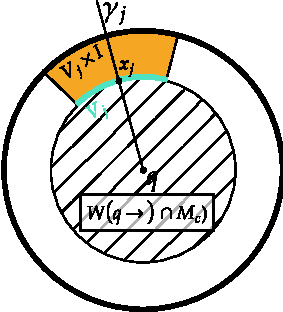
\includegraphics[width=3.8cm]{Text/Pictures/V_jTimesI}}% get height and width
			\hangafter \numexpr -\ht0/\baselineskip -1\relax% adds one blank lines at bottom
			\hangindent \dimexpr \wd0 + 1.2em\relax% adds 1em margin on right
			\vbox{\raisebox{-\height}[0pt][0pt]{\hspace{0.2em}\box0}}\vspace{-1.2ex}% overlap image
			For this we make use of an collar neighbourhood of $W(q\to )\cap M_c$ defined as follows:	Again using the implicit funktion theorem and spherical coordinates (compare \color{red}referenz \color{black}) we have that the preimage of $W(q\to )\cap M_c$ under the embeddign $E^u_q: T^u_qM\to W(q\to)$ is (after rescaling the funktion) a Disk, So withour restrictions assume that $E^u_q(B_1(0))=W(q\to )\cap M_c$. Then $\mathfrak{C}\coloneq E^u_p(B_2(0))$ is a collar neighbourhood and $V_j\times I\hookrightarrow L_i\subseteq \mathfrak{C}$ embedds in the obvious way. This is done by mapping $V_j\times I$ fisrst into $B_2(0)$ via $(v,t)\mapsto (E^u_q)^{-1}v\cdot (1+t)$ and then applying $E^u_p$. 
		\end{minipage}
		
		This mapping $E^u_q$ gives also rise to an oriented chart of $V_j$: For this we deform $B_2(0)$ to be a cylinder along $\gamma_j$ by changing the base such that $(E^u_q)^{-1}x_j$ is the first base vector whilst keeping the orientation ($\det$ of base change is one). Then just strech the disc:
		\begin{equation*}
			(x_1,\dots x_{\lambda_{p}+1})\mapsto (\frac{x_1}{|x_1|},\dots x_{\lambda_{p}+1})\, .
		\end{equation*}. By transversality of $V_j$ and $\gamma_j$ we can assume that the orthogonal projection $\Pi_j$ along the first basis vector restricted to the preimage of $V_j$ is a homeomorphism. Now we get the chart as a composition:
		\begin{align*}
			E^u_{q,j}\coloneq  \Pi_j\circ (E^u_{q})^{-1}: V_j \to \R^{\lambda_{p}} 
		\end{align*}
		Here is where the definition of the Morse boundary operator comes because now we have two different orientations in $V_j$. One induced from $T^u_pM$ (lets call the oriented basis $b^u_p$) and one induced from above. Hence in $Tx_j\gamma_j\oplus Tx_jV_j$ we have two different oriented basis induced from this chart and from the chart given by the tubular neighbourhood embedding of $W(\to p)\cap M^c$ restricted to the normal fiber above $x_j$.
		\begin{center}
			% https://tikzcd.yichuanshen.de/#N4Igdg9gJgpgziAXAbVABwnAlgFyxMJZABgBpiBdUkANwEMAbAVxiRAB12AlAPWE4Z0AtgCModAPpoAviGml0mXPkIoAjOSq1GLNgBUeTKQFk5CkBmx4CRMmq31mrRCABqEgFZytMKAHN4IlAAMwAnCCEkDRAcCCQyEEERGAYABSVrVRAsMGxYEGpHXRcARwlgEUMpWXkQ8MjEACZqWKjCnWcQAClOESw-AB9ygFVygA9PaWk+AFo1WWoklPSrFTZQ-oALHDM6iKRmmLjEBKLOgAoAUSrgEo9pAEoCxLpktIy1lwYYYJ3pCmkQA
			\begin{tikzcd}
				\R^{\lambda_p}                                                   & T^u_pM \arrow[l, "q_{b^u_p}" description] \\
				V_j \arrow[ru, "J\big|_{U_{x_j}}^{-1}"'] \arrow[u, "(E^u_{qj})"] &                                          
			\end{tikzcd}
		\end{center}
		If we now swich to the Alexandrof kompakitifikations we have that this diagramm kommutes up to homotopy, if and only if the orientaions agree. \todo{hier beweis nachholen. Sollte eine einfache übuingsaufgabe sein mittels abbildungsgrad zwischen sphären ist homotopieinvariante}. Else we have a change of sign. Hence we have the diagramm that commutes up to sign: 
		
		\begin{center}	
			% https://tikzcd.yichuanshen.de/#N4Igdg9gJgpgziAXAbVABwnAlgFyxMJZABgBpiBdUkANwEMAbAVxiRAGUAdTmmGAAnYA9YNwZ0AtgCModAPpoAviEWl0mXPkIoAjOSq1GLNtwBmAJzoBjYAGE5O-gBUhTBQFlFozmjrm8jPz2ji5uaJ4qaiAY2HgERGQ6BvTMrIggZpY2wfwAanIAVl7cvv5YgTn5RSoGMFAA5vBEoBYQEkh6IDgQSGQg4lIwDAAKGnHaIOZY9QAWOCDUKcbp3FhQ-Ny8AgCOcsBSrgrKqi3mbUgATNTdHYtGaRmcaxucEGjMcPwAUtxS0wA+ewAqnsAB6FRSKEQAWh0ymoAyGo1iWjYU1m8xOIFa7UQVy6PUQfSWD1W602fH4AAoAKKHYDbIoASgW-TogxGY1R6QYMFMmIoiiAA
			\begin{tikzcd}
				S\vee S^{\lambda_p}                                                                                               & \frac{C_1 T^u_pM}{\partial C_1 T^u_pM} \arrow[l, "\id \vee q_{b^u_p}"'] \\
				\frac{C_1 V_j}{\partial C_1 V_j} \arrow[ru, "\id \oplus J\big|_{U_{x_j}}^{-1}"'] \arrow[u, "\id \vee (E^u_{qj})"] &                                                                        
			\end{tikzcd}
		\end{center}
		
		Here the right path coincides with the path $f_2\circ f_1$. Now we introduce a left part that will later factor over the collaps that induces $\kappa_j$:
		\begin{center}
			% https://tikzcd.yichuanshen.de/#N4Igdg9gJgpgziAXAbVABwnAlgFyxMJZARgBoAGAXVJADcBDAGwFcYkQBlAHS9phgAEHAHrAejegFsARlHoB9NAF8QS0uky58hFACYK1Ok1bseAMwBO9AMbAAwvOICAKsOaKAskrFc09C3hMAg5Oru5oXqrqIBjYeAREZMSGDCxsiCDmVrYhAgBq8gBW3jx+AVhBuQXFURpx2kTkBjSpJhkAcvIAjiEAFAAy3QCUqoYwUADm8ESglhCSSE0gOBBIZCAS0jCMAAqa8TogWGDYsCAtxumZXFhQAjx8gtJuirUgcwuI6ytI+kZpphudx4EDQLDgAgAUjxpFgJgAfeTAACqSIAHkUlCo1LMLPNFjQfog-q0rjxbvdePwBL0AKIvYBdYpDUQAWmIKhom22e3qCQyFjhAAscG8PgTlqtEABmC4AjJmeQAVnOG3oW12+waAuFopx7zxn1lkt+NC2YCgSFZ0qWpPY1ggjAkaAQXPVPK1-JAgomItGSiAA
			\begin{tikzcd}
				N_qC_1(L_q) \arrow[rd, "collaps"', bend right] & S\vee S^{\lambda_p} \arrow[r, "\id \vee b^u_p" description] \arrow[d, "\id \vee (E^u_{qj})^{-1}"'] \arrow[l, "f_5"'] & \frac{C_1 T^u_pM}{\partial C_1 T^u_pM} \arrow[ld, "\id \oplus J\big|_{U_{x_j}}"] \\
				& \frac{C_1 V_j}{\partial C_1 V_j}                                                                                     &                                                                                 
			\end{tikzcd}
		\end{center}
		We define $f_5$ as follows:
		\begin{align*}
			f_5: S\vee S^{\lambda_p}= \frac{B_2(0)}{\partial B_2(0)} &\to N_qC_1(L_q)\\
			x&\mapsto \begin{cases}
				E^u_q(x)& \text{if } \norm{x}\leq 1\\
				(\lambda,x_j)& \text{if } x=(\lambda+1)\cdot x_j\text{, where }\lambda>0 \text{ and }x_j\in 	(E^u_q)^{-1}(V_j)\\
				p& \text{ else}.
			\end{cases}
		\end{align*}
		Now the left side commutes and also factos over the collaps that induces $\kappa_j$.\textit{ hence $\kappa_j$ is up to homotopie the plus or minus the identity which is determined by the sign of the Morse boundary operator at $\gamma_j$}. Now lets collect all:
		
		The (trivialized) tubular neighbourhood embedding 
		\begin{align*}
			J: W(p\to)\cap M^c\cong W(p\to)\cap M^c\times T^u_pM \to N_p
		\end{align*}
		together with collapsing $W(\to p)\cap M^c$ (which is realiced by the projection $\pi: W(p\to)\cap M^c\times T^u_pM\to T^u_pM$) and a koordinate map $q$ induced by a basis of $T^u_pM$ gives rise to a map:
		\begin{align*}
			T\coloneq q_{b^u_p}\circ \pi\circ J^{-1}: N_p\to \R^{\lambda_{p}}
		\end{align*}
		This gives rise to a well defined map 
		\begin{equation*}
			\tilde{T}: \frac{N_p}{L_p}\to \overline{\R^{\lambda_{p}}}\cong S^{\lambda_p}; \tilde{T}(x)=\overline{T(x)}
		\end{equation*}which again can be extended to a map which we will call $T$ by abuse of notation: 
		\begin{align*}
			T\coloneq \id\vee \tilde{T}: S_1\vee \left(L_q\cup N_p \middle/  L_p \cup \cl (L_q \setminus {N_p})\right) \to S^{\lambda_p+1}
		\end{align*} 
		
		Hence, the Morse datum together with $T$ gives rise to a natural generaor of $K^{\lambda_p-1}\left[L_q\cup N_p ,  L_p \cup \cl (L_q \setminus {N_p})\right]$. Furthermore the map  $\left((c_j\circ \Lambda)^*\right)_j^{-1}\circ c_{\iota}^*\circ (\eta^*)^{-1}\circ \gamma^*\circ T$ commutes with the map $\id \vee b^u_p\circ (\id \oplus J\big|_{U_{x_j}})$. To see this notice how $\eta$ and $\gamma$ are just the identity. Furthermore $c_\iota$ is, and $\left((c_j\circ \Lambda)^*\right)_j^{-1}$ is induced by the inclusion of $C_1V_j\big/ \partial C_1V_j$ into the space $C_1L_q\big/ \cl\left(C_1(L_q)\setminus \bigcup\limits_{j=1}^lC_1V_j \right)$. Hence the composition reads
		\begin{align*}
			\left((c_j\circ \Lambda)^*\right)_j^{-1}\circ c_{\iota}^*\circ (\eta^*)^{-1}\circ \gamma^*
			=\left(\gamma \circ \eta^{-1}\circ c_{\iota}\circ i\right)^*\\
			=\left[x\mapsto \begin{cases}
				p & \text{ if }x\in N_q\cup N_p\cup C_1\left(L_q\cup \cl\left(L_q\setminus \bigcup\limits_{j=1}^lV_j\right) \right)\\
				x & \text{ else .}
			\end{cases}\right]^*
		\end{align*}  Now the collapsing reqirement is much easyer in reality, is $x$ comes from $C_1V_j$ because: 
		\begin{align*}
			C_1V_j \bigcup N_q\cup N_p\cup C_1\left(L_q\cup \cl\left(L_q\setminus \bigcup\limits_{j=1}^lV_j\right) \right)= \partial C_1V_j 
		\end{align*} With this in mind, the whole composition equals:
		\begin{align*}
			q_{b^u_p}\circ \pi \circ J^{-1}\circ \gamma \circ \eta^{-1}\circ c_{\iota}\circ i=(\id \vee q_{b^u_p})\circ (\id \oplus J^{-1}) \, .
		\end{align*}
		Hence this composition equals $(id\vee J\big|_{U_{x_j}}\circ B_{b^u_p})^{-1}$. Now lets stich everything together and let $p$ be a generator of $K^{\lambda_p-1}\left[L_q\cup N_p ,  L_p \cup \cl (L_q \setminus {N_p})\right]$ induced by $T$ and the orientation of $T^u_pM$. (This means that $p=T^*(\beta)$, where $\beta$ is the Bott generator of $K^{\lambda_p-1}[S^{\lambda_p-1}]$). Then:
		\begin{align*}
			\delta_{triple}(p)
			&=(m^*)^{-1}\circ \underbrace{c^*\circ i_{\delta}^*\circ i_{\eta}^*}_{=\sum\limits_{j=1}^l\kappa _j\circ \pi_j}\circ c_{\iota}^*\circ (i_{\eta}^{-1})^*\circ \gamma^*(p)\\
			&=(m^*)^{-1} \circ \sum_{j=1}^{l}\left(\kappa_j\circ \pi_j\circ c_{\iota}^*\circ (i_{\eta}^{-1})^*\circ \gamma^*\right)(T^*(\beta))\\
			&=(m^*)^{-1} \circ \sum_{j=1}^{l}\left(\kappa_j\circ (\underbrace{q_{b^u_p}\circ \pi\circ J^{-1}\circ \gamma \circ i_{\eta}^{-1}\circ c_{\iota}\circ i_j}_{=(\id \vee q_{b^u_p})\circ (\id \oplus J^{-1})})^*(\beta)\right)\\
			&=(m^*)^{-1} \circ \sum_{j=1}^{l}\left(\kappa_j((\pm)_{\gamma_j}(\id\vee E^u_{qj})^*(\beta)) \right)
		\end{align*}
		Now we give its image a canonical generator induced by a basis of $T^u_qM$. For this we need a map $S^{\lambda_p+1}\to N_q\big/ L_q$ that commutes with $(m^*)^{-1} \circ f_5$. Once we have this we are finally done!!!
		This however can be done easily. For this we make use of the unstable manifold theorem and rescale the immersion such that $W(q\to )\cap M_c$ is the image of the Ball $B_0(1)$. Furthermore,  $N_q\slash L_q\simeq W(q\to )\cap M_c$ since it is a tubular neighbourhood. Hence we get a map 
		\begin{align*}
			(E^u_q):  S^{\lambda_p+1}\to N_q\slash L_q
		\end{align*} Now $(E^u_q)\simeq (m\circ f_5)\simeq \id$ since  $(E^u_q)^{-1}\circ (m\circ f_5)\simeq \id$. The latter is clear due to the first being just a streching $B_0(1)\to B_0(2)$ and then collaps of the outer ring. This composition however obvieously is homotopic to the identity. 
		Hence $(E^u_q)^*\circ (m^*)^{-1}=f_5^*$ .
		
		Now we apply $(E^u_q)^*$ to the calculation above to figure out the map:
		
		\begin{align*}
			(E^u_q)^*\circ 	\delta_{triple}(p)
			&= (E^u_q)^*\circ (m^*)^{-1} \circ \sum_{j=1}^{l}\left(collaps^* \circ (\pm)_{\gamma_j} (\id\vee E^u_{qj})^*(\beta) \right)\\
			&= \sum_{j=1}^l (\pm)_{\gamma_j} f_5^* collaps^* \circ (\id\vee E^u_{qj})^*(\beta)\\
			&=\sum_{j=1}^l (\pm)_{\gamma_j} \beta=n(p,q)\beta
		\end{align*}
		Or said differently by defining $q$ to be the generator of $N_q\big/L_q$ given by the orientation of $T^u_qM$ as $q=((E^u_q)^{-1})^*(\beta)$ then:
		\begin{equation*}
			\delta_{triple}(p)=n(p,q)q\,.
		\end{equation*} 	
		\todo{Uns interresiert wie viele q da rauskommen. Also eher eine Koordinatenmap nach dem tripple operator. Wenn ich die einfüre,dann könnte es passen? }
		
		
		% https://tikzcd.yichuanshen.de/#N4Igdg9gJgpgziAXAbVABwnAlgFyxMJZABgBoAmAXVJADcBDAGwFcYkQBpAPTQAIAdHIP79GMAGY5kvGcKFD+4gE70AxsF4BhAPoBGABQAZbQEcAlAF8B8ubw0jVjWTfnWRYyfrcvvOg8fMROBgcAFssMGY4AX4AIywAc1VmNHcscJw4bWAAKwBeXQsuJz8ANW0c5zlBN34lRIALHDMqnytqusacShALUnRMXHxCFF0KajomVnZuVNEJKTKKmPiEgHoYtHolPCYtPV5ynJF6hKaevoHsPAIiMl0JhhY2RE4edwXkADlTBxTeH5zZJ8PxGX78YEA7RoMwnLoXfogDDXYZEcikB40J7TV6zD6SZB+AAqXGY0IAsitEhsRFsdlg9n5eCSyWhKXCzt1eojkUNbigyMRHlMXm85h4pD8TFT1mDAp1OQirnyRsgxkKsSKZjxkAARUnZEQwNDYRgECwiVZrWnbXZOfVk4BGk1YM1gKxKpGDG6q9EaybPbVoZAAZS4TtE9FCsSg9GhAGpCp7eT6iGNMQGcWLkCJlGpgAAhbTkfTESwRul23hFktliwXCYwKAJeBEUDKCChJBkEA4CBIciXEAdruIMa9-uIdGZ0UiADW9DQWxANEY9FiMEYAAVvajXqcmtz20pO0hx33u0OR0gAMw0C9jzWB17iYtH4cn0fTh8AFivn6QH970nABWf9T0QEDgKQAA2J8s1fH932vKdoMg+DRVfG9kIAxA4InW8MPYV9dBwiCAHY0LvGd2FiPQyNHSiCPQmjXjo8gVxAOAGiwSRL0RFCmIfcdsVneZPH0ABRA1zHDABaQoHCwJRVF4LAOSaMwuAAKk4tcN23Xd+RACJsFgXpKAsIA
		\begin{tikzcd}
			{K^p\left[N_q \big/(L_q)\right]} \arrow[r]                                                                                                                      & {K^p[D^u_{\epsilon}\big/\partial D^u_{\epsilon} ]} \arrow[r, "f_4"]                                                                 & {K^p[S^{\lambda_p+1}]} \arrow[d, "f_1"]                                  \\
			{K^p\left[N_q\cup N_p\cup C_1(L_q\cup N_p)\right]} \arrow[u] \arrow[ru, "f_3"]                                                                                  & {K^p[\frac{B_2(0)}{\partial B_2(0)}]} \arrow[r, "b_1"] \arrow[u, "b_2"] \arrow[d, "\left((E^u_q)^{-1}\circ i\right)^*" description] & {K^p\left[C_1T^u_pM \big/ \partial C_1 T^u_pM \right]} \arrow[ld, "f_2"] \\
			{K^p 		\left[   			\frac{ C_1(L_q)} 				 { \cl  				 	\left( 				 		C_1(L_q)\setminus \bigcup\limits_{j=1}^l C_1V_j  				 	\right)  				 } 		\right]} \arrow[u] & {K^p\left[C_1V_j \big/ \partial C_1 V_j\right]} \arrow[lu, "\kappa_j"'] \arrow[l]                                                     &                                                                         
		\end{tikzcd}
		Now we start going arround that diagramm wich is commutative up to hopotopie and start at the bottom. $b_1$ is the same map as $f_1$ and hence makes use of the orientation of $T^u_pM$. $f_2\circ b_1$ is homotopic to the inculsion induced mapping $\left((E^u_q)^{-1}\circ i\right)^*$. This can be seen as follows: First notice how $f_2\circ b_1$ is homotopic to map induced from $(\id\oplus E^u_{q,j})^{-1})$
		\begin{equation*}
			(x_1,\dots x_{\lambda_{p}+1})\mapsto (\frac{x_1}{|x_1|},\dots x_{\lambda_{p}+1})\, .
		\end{equation*}
		now the half cylinder ($x_1\geq 0$) is again homotopic to the whole with the inclusion and collapsing being the homotopic invers maps. Those considerations also work modulo the boundary. Now $f_2\circ b_1$ is homotopic to $\left((E^u_q)^{-1}\circ i\right)^*$ if and only if the chart $(E^u_q)^{-1}$  by applying the streching map $s:\frac{B_2(0)}{\partial B_2(0)}\to \frac{B_2(0)}{\partial B_2(0)}$: (which is homotopic to the identity.)
		\begin{center}
			
			
			\tikzset{every picture/.style={line width=0.75pt}} %set default line width to 0.75pt        
			
			\begin{tikzpicture}[x=0.75pt,y=0.75pt,yscale=-1,xscale=1]
				%uncomment if require: \path (0,300); %set diagram left start at 0, and has height of 300
				
				%Shape: Block Arc [id:dp2516942430671658] 
				\draw  [fill={rgb, 255:red, 245; green, 166; blue, 35 }  ,fill opacity=1 ] (284,83.96) .. controls (298.88,68.69) and (319.24,58.69) .. (342.17,57.27) .. controls (351.83,56.67) and (361.22,57.63) .. (370.11,59.95) -- (362.53,89.26) .. controls (356.65,87.73) and (350.44,87.08) .. (344.05,87.48) .. controls (328.89,88.42) and (315.43,95.05) .. (305.6,105.17) -- cycle ;
				%Shape: Ellipse [id:dp31830895843634066] 
				\draw  [line width=2.25]  (258.59,146.8) .. controls (258.59,97.56) and (298.5,57.65) .. (347.74,57.65) .. controls (396.97,57.65) and (436.89,97.56) .. (436.89,146.8) .. controls (436.89,196.04) and (396.97,235.95) .. (347.74,235.95) .. controls (298.5,235.95) and (258.59,196.04) .. (258.59,146.8) -- cycle ;
				%Shape: Ellipse [id:dp9709870130157104] 
				\draw   (288.6,146.8) .. controls (288.6,114.14) and (315.08,87.66) .. (347.74,87.66) .. controls (380.4,87.66) and (406.87,114.14) .. (406.87,146.8) .. controls (406.87,179.46) and (380.4,205.93) .. (347.74,205.93) .. controls (315.08,205.93) and (288.6,179.46) .. (288.6,146.8) -- cycle ;
				%Shape: Circle [id:dp482439832706389] 
				\draw  [draw opacity=0][fill={rgb, 255:red, 0; green, 0; blue, 0 }  ,fill opacity=1 ] (348.7,143.89) .. controls (349.7,143.43) and (350.88,143.87) .. (351.33,144.87) .. controls (351.79,145.87) and (351.35,147.04) .. (350.35,147.5) .. controls (349.35,147.95) and (348.17,147.51) .. (347.72,146.51) .. controls (347.27,145.52) and (347.71,144.34) .. (348.7,143.89) -- cycle ;
				%Shape: Arc [id:dp1835190035098445] 
				\draw  [draw opacity=0][line width=2.25]  (305.17,104.91) .. controls (315.42,94.49) and (329.49,87.79) .. (345.25,87.13) .. controls (351.39,86.87) and (357.36,87.55) .. (363.01,89.04) -- (347.74,146.8) -- cycle ; \draw  [color={rgb, 255:red, 80) -- (423.42,97.86) ;
					%Straight Lines [id:da15646287377542745] 
					\draw    (320.32,61.14) -- (397.42,70.86) ;
					
					%Straight Lines [id:da5095357448746147] 
					\draw    (323.57,61.6) -- (351.75,235.79) ;
					%Straight Lines [id:da6233786094876668] 
					\draw    (323.57,61.6) -- (321.84,230.24) ;
					%Straight Lines [id:da23916661666457828] 
					\draw    (322.57,62.6) -- (289.95,214.07) ;
					%Straight Lines [id:da33960840190709396] 
					\draw    (322.57,62.6) -- (270.05,186.5) ;
					%Straight Lines [id:da11039605607469682] 
					\draw    (322.57,62.6) -- (260.47,152.72) ;
					%Straight Lines [id:da5150377253833407] 
					\draw    (322.57,62.6) -- (265.75,115.61) ;
					
					% Text Node
					\draw (311.67,43.4) node [anchor=north west][inner sep=0.75pt]  [font=\scriptsize]  {$y_{j}$};
					
					
				\end{tikzpicture}
				
			\end{center}
			Using this streching we have that 
			\begin{minipage}{\dimexpr \textwidth-2\fboxsep-2\fboxrule}
				\abovecaptionskip=0pt
				\sbox0{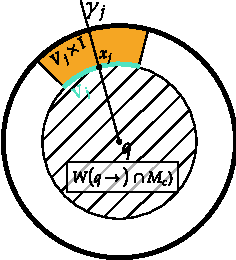
\includegraphics[width=3.8cm]{Text/Pictures/the rescaling with rays}}% get height and width
				\hangafter \numexpr -\ht0/\baselineskip -1\relax% adds one blank lines at bottom
				\hangindent \dimexpr \wd0 + 1.2em\relax% adds 1em margin on right
				\vbox{\raisebox{-\height}[0pt][0pt]{\hspace{0.2em}\box0}}\vspace{-1ex}% overlap image
				Furthermore, $V_j\times I$ is homeomorphic to $\mathfrak{C}$ by streching it. The streching can be done along rays starting in $y_j=(x_j,1)$. This is homotopic to the identity, if viewed as a endomorphism in $W(q\to)\cap M_c$. We can now define the collapsing map $W(q\to)\cap M_c$ in a continouos way by defining it to be the identity inside of $L_j$ and outside we map each point to the intersection of the ray containing said point with the bundary of $L_p$.
				Das solworklte die letzte Lücke sein!
			\end{minipage}
		\end{proof}; green, 227; blue, 194 }  ,draw opacity=1 ][line width=2.25]  (305.17,104.91) .. controls (315.42,94.49) and (329.49,87.79) .. (345.25,87.13) .. controls (351.39,86.87) and (357.36,87.55) .. (363.01,89.04) ;  
	%Shape: Ellipse [id:dp3336819844491399] 
	\draw  [draw opacity=0][fill={rgb, 255:red, 0; green, 0; blue, 0 }  ,fill opacity=1 ] (331.4,87.95) .. controls (332.4,87.49) and (333.57,87.93) .. (334.03,88.93) .. controls (334.48,89.93) and (334.04,91.11) .. (333.04,91.56) .. controls (332.05,92.02) and (330.87,91.58) .. (330.41,90.58) .. controls (329.96,89.58) and (330.4,88.4) .. (331.4,87.95) -- cycle ;
	%Straight Lines [id:da2883617960271355] 
	\draw    (320.32,61.14) -- (375.42,231.86) ;
	%Straight Lines [id:da6580977928561076] 
	\draw    (320.32,61.14) -- (399.42,218.86) ;
	%Straight Lines [id:da549347805026984] 
	\draw    (320.32,61.14) -- (420.42,196.86) ;
	%Straight Lines [id:da3542746287685834] 
	\draw    (320.32,61.14) -- (435.42,164.86) ;
	%Straight Lines [id:da38915223346361993] 
	\draw    (320.32,61.14) -- (435.42,130.86) ;
	%Straight Lines [id:da011207389658813405] 
	\draw    (320.32,61.14



